%%%%%%%%%%%%%%%%%%%%%%%%%%%%%%%%%%%%%%%%%%%%%%%%%%%%%%%%%%%%%%%%%%%
%
% Flageul C., Tiselj I., Benhamadouche S., Ferrand M.
% https://doi.org/10.1007/s10494-019-00008-0
%
%%%%%%%%%%%%%%%%%%%%%%%%%%%%%%%%%%%%%%%%%%%%%%%%%%%%%%%%%%%%%%%%%%%

\RequirePackage{fix-cm}

\documentclass{svjour3}                     % onecolumn (standard format)
%\documentclass[smallcondensed]{svjour3}     % onecolumn (ditto)
%\documentclass[smallextended]{svjour3}       % onecolumn (second format)
%\documentclass[twocolumn]{svjour3}          % twocolumn

\smartqed  % flush right qed marks, e.g. at end of proof

\usepackage{tikz}
\usepackage{textcomp}
\usepackage{hyperref}
\usepackage{multirow}
\usepackage{graphicx}
%
\usepackage{mathptmx}      % use Times fonts if available on your TeX system
%
% insert here the call for the packages your document requires
%\usepackage{latexsym}
\usepackage{mathtools}
\usepackage{lineno}
\linenumbers

% please place your own definitions here and don't use \def but
% \newcommand{}{}

% Insert the name of "your journal" with
\journalname{Flow, Turbulence and Combustion}
%
\begin{document}

\title{A correlation for the discontinuity of the temperature variance dissipation rate at the fluid-solid interface in turbulent channel flows%\thanks{Grants or other notes
%about the article that should go on the front page should be
%placed here. General acknowledgments should be placed at the end of the article.}
}
%\subtitle{Do you have a subtitle?\\ If so, write it here}

\titlerunning{LES of a turbulent channel flow : A correlation for $\varepsilon_\theta$ at the fluid-solid interface} % if too long for running head

\author{C\'edric Flageul \and
        Iztok Tiselj \and
        Sofiane Benhamadouche \and
        Martin Ferrand
}

\authorrunning{C. Flageul, I. Tiselj, S. Benhamadouche, M. Ferrand} % if too long for running head

\institute{C. Flageul \and I. Tiselj \at
              Institut Jo\v{z}ef Stefan, Reactor Engineering Division, Slovenia \\
              \email{cedric.flageul@ijs.si}
           \and
           S. Benhamadouche \and M. Ferrand \at
              EDF R\&D, Fluid Mechanics, Energy and Environment Department, France \\
              \email{sofiane.benhamadouche@edf.fr}
}

\date{Received: date / Accepted: date}
% The correct dates will be entered by the editor

\maketitle

\begin{abstract}
Discontinuity of the dissipation rate associated with the temperature variance at the fluid-solid interface is analyzed in a turbulent channel flow at a Reynolds number, based on the friction velocity of 395 and a Prandtl number of 0.71.
The analysis is  performed with a wall-resolved Large Eddy Simulation and the results are used to derive a regression for the dissipation rate discontinuity, which depends only on the fluid-solid thermal diffusivity and conductivity ratios.
Wall-resolved Large Eddy Simulations at a higher Reynolds number and a higher Prandtl number are used to investigate the validity of two correlations derived from the regression for the selected thermal properties ratios.
The present results are obtained with the open-source Computational Fluid Dynamics solver {\fontfamily{ppl}\fontshape{it}\selectfont Code\_Saturne}, and use the fully conservative fluid-solid thermal coupling capability introduced by the authors in version 5.0.
\end{abstract}

\section{Introduction}
\label{sec-introduction}

Conjugate heat transfer refers to the thermal coupling between a fluid and a surrounding solid.
It is of prime importance in industrial applications where thermal fatigue is a concern.
In the nuclear field, thermal fatigue and fluctuating thermal stresses are particularly important in case of a severe emergency core cooling or long-term ageing of materials.
Such complex applications are often studied experimentally and numerically.
However, numerical investigations of turbulent flows at moderate to high Reynolds numbers remain challenging.
CFD (Computational Fluid Dynamics) analysis of industrial applications usually relies on high or low Reynolds RANS (Reynolds-Averaged Navier-Stokes) and occasionally on wall-modelled LES (Large Eddy Simulation) for the low to moderate Reynolds numbers (Benhamadouche \cite{benhamadouche2017ned}, Hassan \cite {hassan2017overview}).

The turbulent flow applies on the solid domain a thermal load characterized by a broad spectrum.
Qualitatively, the heat diffusion in the solid domain provides a strong damping at high frequencies.
Therefore, smaller scales tend to apply a thermal stress in the vicinity of the fluid-solid interface while larger scales tend to penetrate deeper in the solid.
Refined analysis actually shows that high stress amplitude events are generally associated with low probability ones (Costa Garrido et al. \cite{garrido2016uncertainties}), thus making accurate estimation of thermal fatigue in industrial applications even more challenging as the CFD simulations should provide at least a few minutes of operation in realistic conditions.

Analytical studies on conjugate heat transfer in turbulent flows were pioneered by Polyakov \cite{poliakov1974wall} and Geshev \cite{geshev1978influence}.
The fundamental solutions of the heat equation in the solid domain have a non-compact support.
For instance, semi-infinite solids with a flat fluid-solid interface subjected to a statistically steady forcing can be characterized by a compatibility condition at the fluid-solid interface expressed as a spatio-temporal convolution (Flageul et al. \cite{flageul2015dns}).
Such non-local effects are specific to conjugate heat transfer and tend to become negligible only when the thermal properties of the fluid and of the solid differ by orders of magnitude.

Numerical studies on conjugate heat transfer in turbulent flows were pioneered by Kasagi et al. \cite{kasagi1989numerical} and their 2D synthetic turbulence model.
The first DNS (Direct Numerical Simulation) with conjugate heat transfer was a turbulent channel flow, performed by Tiselj et al. \cite{tiselj2001dns}.
Following those studies, some of the present authors and co-workers performed additional DNS of the turbulent channel flow \cite{flageul2015dns} to extract the budgets of the second moments (i.e. the turbulent heat fluxes and the temperature variance).
This work was motivated by the global lack of validation data for second-order RANS turbulence models (Dehoux et al. \cite{dehoux2017elliptic}, \cite{dehoux2012algebraic}) in case of an imposed heat flux, in case of a heat exchange coefficient, or in case of conjugate heat transfer, most of the previous DNS of the turbulent channel flow using an imposed temperature at the wall (Kasagi et al. \cite{kasagi1992direct}, Kawamura et al. \cite{kawamura1998dns}, Abe et al. \cite{abe2004surface}).%, which corresponds to a Dirichlet boundary condition.

To the best of the authors knowledge, the only RANS turbulence model designed to take into account conjugate heat transfer --- i.e. able to solve the temperature fluctuations both in the fluid and in the solid --- was published by Craft et al. \cite{craft2010towards}.
It is also the only RANS turbulence model designed to correctly handle cases with an imposed heat flux (Mangeon et al. \cite{mangeon2018thmt}).
However, it was recently shown that the dissipation rate ($\varepsilon_\theta$) associated with the halved temperature variance ($\overline{{T'}^2} / 2$) is discontinuous at the fluid-solid interface in case of conjugate heat transfer (Flageul et al. \cite{flageul2017discontinuity}).
Although there is currently no coupled RANS model taking this discontinuity in account there is a global agreement that one is needed (Shams et al. \cite{shams2018synthesis}).

The background on such turbulence models is given in the paper of Craft et al. \cite{craft2010towards} and in classic textbooks on turbulence modelling (Hinze \cite{hinze_turbulence}, Pope \cite{pope_turbulent}, Leschziner \cite{leschziner_turbulence}).
A simple --- and thus approximate --- sketch would be to say that RANS models use the turbulent kinetic energy $k$ and the associated dissipation rate $\varepsilon$ to model velocity fluctuations.
Regarding temperature fluctuations, the halved temperature variance $\overline{T'^2}/2$ and the associated dissipation rate $\varepsilon_\theta$ are very similar to $k$ and $\varepsilon$, respectively.
However, velocity fluctuations remain inside the fluid domain while temperature fluctuations may penetrate inside solid domains adjacent to the fluid one.
In case of conjugate heat transfer, this fundamental difference must be taken into account, and the turbulence model should be able to evaluate $\overline{T'^2}$ and $\varepsilon_\theta$ in the solid domain adjacent to the fluid one.

The objectives of this paper are twofold.
First, we present the new stand-alone fluid-solid thermal coupling capability implemented in the open-source CFD code {\fontfamily{ppl}\fontshape{it}\selectfont Code\_Saturne}\footnote{See \url{https://www.code-saturne.org}}, we use it to perform wall-resolved LES of the turbulent channel flow with conjugate heat transfer at moderate Reynolds numbers and we assess the results using DNS.
The objective of this first step is to expose and validate our developments.
Second, we perform and analyse various wall-resolved LES with conjugate heat transfer at a higher Reynolds and Prandtl numbers, and with various ratios of fluid-solid thermal properties.
The objective of this second step is to investigate their respective influence on the discontinuity of $\varepsilon_\theta$ at the fluid-solid interface.
The correlations we propose for the discontinuity of $\varepsilon_\theta$ are the outcome of this second step.
Indeed, the correlations proposed are expected to be valid only for the range of fluid-solid thermal properties ratio investigated, and for turbulent flows similar to the one simulated.
However, the methodology used being generic, it could potentially be applied to any configuration of interest, provided one can perform wall-resolved LES of this configuration.

The present paper is divided into five sections.
Section \ref{sec-gov_eq_geom} presents the governing equations and describes the turbulent channel flows investigated.
Section \ref{sec-discret} presents the discretisation used to solve the governing equations alongside with the extrapolation of statistics performed at the fluid-solid interface.
Section \ref{sec-valid} presents the validation of our wall-resolved LES against DNS.
Section \ref{sec-higher} presents some new LES results and our correlations for the discontinuity of $\varepsilon_\theta$.
Ultimately, in Section \ref{sec-disc_conclu}, our results are further discussed, alongside with some concluding remarks and some perspectives.
%{\color{red}The appendix \ref{sec-coupl_strat} presents the fluid-solid thermal coupling strategy implemented.}

\section{Governing equations and cases description}
\label{sec-gov_eq_geom}

\subsection{Governing equations}
\label{subsec-gov_eq}
We consider the turbulent flow of a Newtonian fluid with constant physical properties.
Furthermore, we assume that the flow is incompressible and that the physical properties in the solid domains are also constant.
The subscripts $f$ and $s$ are used for the fluid and for the solid, respectively.

In this subsection, we omit boundary conditions for the sake of simplicity.
Firstly, the conservation of mass in a fluid with a constant density reduces to the incompressibility condition
\begin{equation}
\partial_i u_i = 0
\end{equation}
where $u_i$ and $\partial_i$ are the velocity and the spatial derivative in direction $i$, respectively.

Secondly, the conservation of momentum in the fluid domain is
\begin{equation}
\partial_t u_i + \partial_j \left( u_i u_j \right) = - \frac{1}{\rho_f} \partial_i P + \partial_j \sigma_{ij} + f_i
\end{equation}
where $\partial_t$ is the time derivative, $\rho$ the density, $P$ the dynamic pressure, $\sigma_{ij}$ the deviatoric part of the stress tensor and $f_i$ a source term.
We use the WALE subgrid-scale model (Nicoud and Ducros \cite{nicoud1999subgrid}) as implemented in the version 5.0 of {\fontfamily{ppl}\fontshape{it}\selectfont Code\_Saturne}: ${\sigma_{ij} = \left( \nu + \nu_t \right) S_{ij}}$ with
\begin{equation}
\nu_t = 4 \sqrt{2} V_{cell}^{2/3} C_w^2 \frac{\left(S_{kl}^dS_{kl}^d\right)^{5/4}}{\left(S_{kl}S_{kl}\right)^{5/2} + \left(S_{kl}^dS_{kl}^d\right)^{5/4}} 
\end{equation}
where $\nu$ is the kinematic viscosity, $V_{cell}$ the volume of the computational cell, $C_w$ the model constant, $S_{ij}^d$ the deviatoric part of the square of $\partial_j u_i$ and $S_{ij}$ the mean strain rate tensor.
The constant $C_w$ is set to 0.25, the default value in {\fontfamily{ppl}\fontshape{it}\selectfont Code\_Saturne}.

Lastly, the energy conservation equation is
\begin{equation}
\partial_t T_f + \partial_i \left( T_f u_i \right) = \partial_j \left( \left( \alpha_f + \frac{\nu_t}{{Pr}_t} \right) \partial_j T_f \right) + f^{T_f}
\end{equation}
in the fluid domain and
\begin{equation}
\partial_t T_s = \alpha_s \partial_{jj} T_s + f^{T_s}
\end{equation}
in the solid domain with
\begin{equation}
T_f = T_s \mbox{ and } \lambda_f \partial_n T_f = \lambda_s \partial_n T_s
\end{equation}
at the fluid-solid interface.
Here, $T$ is the temperature, $\alpha$ the thermal diffusivity, ${Pr}_t$ the turbulent Prandtl number, $f^T$ a source term and $\lambda$ the thermal conductivity.
The turbulent Prandtl number is set to $0.5$ in the present study (Gr\"{o}tzbach \cite{grotzbach2011revisiting}).
Additional simulations were performed to investigate the effect of the SGS model and the impact of $Pr_t$, as exposed in the appendix \ref{sec-sgs_appendix}.
Overall, the impact of the modelling parameter $Pr_t$ is limited to the fluid domain but is null while approaching the fluid solid interface.
Thus, the turbulent Prandtl number has little effect on the target values of the present study.

As we investigate forced convection, the transported scalars --- like the temperature --- do not impact the velocity field or the pressure.
Thus, we can transport simultaneously an arbitrary number of passive scalars, and each scalar can use different thermal properties in the fluid and in the solid.
This allows significant savings in terms of CPU time: each passive scalar is transported by the same velocity field.
This peculiarity has eased our investigation as it reduced the impact of the statistical uncertainty (Flageul and Tiselj \cite{flageul2017impact}).

\subsection{Geometry}
\label{subsec-geom}

Figure \ref{fig-sketch} is a sketch of the domain. $x$, $y$ and $z$ are the streamwise, wall-normal and spanwise directions, respectively.
The fluid domain is bounded (${-\delta < y < \delta}$) and $\delta$ is the channel half-height.
The solid domains on top and on bottom of the fluid one are located at ${y > \delta}$ and ${y < -\delta}$, respectively.
Both have the same total height, $\delta_S$.
The exact extension of the channel in the streamwise and spanwise directions and the height of the solid domains depend on the case considered, as described in Subsection \ref{subsec-simu-done}.
Based on previous studies, the present authors estimate that for all the cases considered here and summarized in Tables \ref{tab-valid-geo} and \ref{tab-higher-geo}, the solid domains extension in the wall-normal direction is sufficient so that the boundary condition used at the outer wall has no significant impact on the statistics at the fluid-solid interface.

\begin{figure}
\centering
%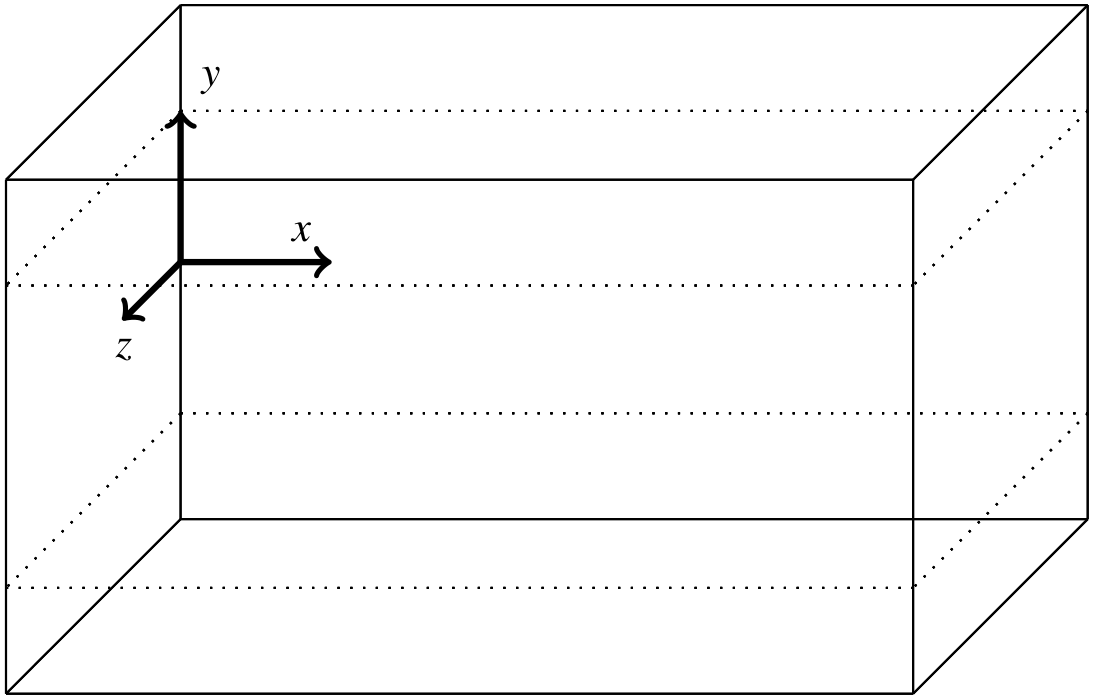
\includegraphics[width=0.5\textwidth]{./images/sketch.png}
  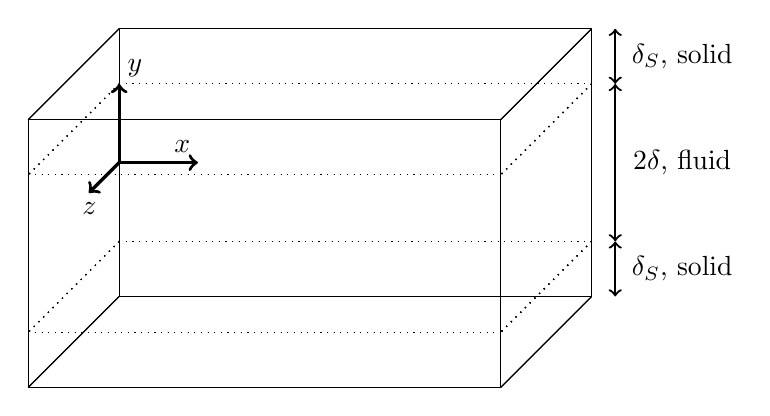
\begin{tikzpicture}
    \draw[thick, <->] (3.3,-1.,0) -- node [] {} (3.3,1.,0);
    \node at (4.15,0.,0) {$2 \delta$, fluid};
    \draw[thick, <->] (3.3,1.7,0) -- node [] {} (3.3,1.,0);
    \node at (4.15,1.35,0) {$\delta_S$, solid};
    \draw[thick, <->] (3.3,-1.7,0) -- node [] {} (3.3,-1.,0);
    \node at (4.15,-1.35,0) {$\delta_S$, solid};
    \draw [very thick,->] (-3,0,0) -- (-2,0,0);
    \draw [very thick,->] (-3,0,0) -- (-3,1,0);
    \draw [very thick,->] (-3,0,0) -- (-3,0,1);
    \node at (-2.2,0.2,0) {$x$};
    \node at (-2.8,1.2,0) {$y$};
    \node at (-2.8,0,1.5) {$z$};
    \foreach \x in{-3,3}
    { \foreach \y in{-1.7,1.7}
    { \foreach \z in{0,3}
    {   \draw (-3,\y,\z) -- (3,\y,\z);
        \draw (\x,-1.7,\z) -- (\x ,1.7,\z);
        \draw (\x,\y,3) -- (\x,\y,0);
        \draw[dotted] (-3,-1.,\z) -- (3,-1.,\z);
        \draw[dotted] (-3,1.,\z) -- (3,1.,\z);
        \draw[dotted] (\x,-1.,0) -- (\x,-1.,3);
        \draw[dotted] (\x,1.,0) -- (\x,1.,3);
    }
    }
    }
  \end{tikzpicture}
\caption{
Channel flow with fluid-solid thermal coupling.
The solid domains are on top (${y>\delta}$) and on bottom (${y<-\delta}$) of the fluid one (${-\delta<y<\delta}$).
Dotted lines: fluid-solid interfaces at ${y = \pm \delta}$.
}\label{fig-sketch}
\end{figure}

For all the LES considered here, the size of the cells in wall-units in the streamwise and spanwise directions is ${\delta x}^+ = 30$ and ${\delta z}^+=15$, respectively.
On both sides of the fluid-solid interfaces, the first cell has an extension in the wall-normal direction of $1$ wall-unit.
Further away from the wall, the wall-normal extension of the cell is bigger, according to a geometric law with a progression factor of $1.09$.
In the fluid, as soon as the wall-normal extension of the cell reaches $15$ wall-units, this progression factor is set to $1$ so that the wall-normal extension of the cells does not exceed their spanwise extension.
All the LES use a constant time step with a maximal instantaneous CFL number around 0.5.

\subsection{Source terms}
\label{subsec-sce_trm}

The source term in the momentum equation in the fluid is an imposed pressure gradient, which is constant in space and in time.
It compensates the viscous friction at the wall and keeps the flow in a statistically steady state.
Using the averaged momentum equation, the no-slip boundary condition and the vanishing $\nu_t$ at the wall, one can derive ${\delta f_x = u_\tau^2}$ where $u_\tau$ is the friction velocity, derived from the wall shear stress.
The Reynolds number based on the friction velocity and the channel half-height is ${Re_\tau = \frac{u_\tau \delta}{\nu}}$.
This definition, combined with the previous relation, allows us to choose the source term $f_x$ so that the target $Re_\tau$ is exactly reached:
\begin{equation}
f_x = \frac{\nu^2 Re_\tau^2}{\delta^3} \mbox{ and } f_y = f_z = 0\mbox{.}
\end{equation}

The source term in the energy equation in the fluid domain depends on the instantaneous streamwise velocity and on the instantaneous bulk velocity, as defined by Kasagi et al. \cite{kasagi1992direct}.
It is a volumetric source term which compensates the heat output at the boundaries, so that the case remains statistically steady.
Using the previous notations and writing $q_w$ the heat flux per unit surface outputted at the top and bottom boundaries, the source term in the energy equation in the fluid domain is:
\begin{equation}
f^{T_f} = \frac{2 \alpha_f q_w L_x L_z}{\lambda_f} \frac{ u_x (x,y,z,t) } {\int_{x=0}^{L_x} \int_{y=-\delta}^\delta \int_{z=0}^{L_z} u_x \,dz \,dy \,dx}
\end{equation}
Subsection \ref{subsec-cond_lim} further describes the boundary conditions used.
There is no source term in the energy equation in the solid domain ($f^{T_s}=0$) since the heating of the solid wall is provided through the constant heat flux imposed at the outer side of the wall.

The source terms used allow one to derive a theoretical friction velocity and friction temperatures which are not plagued by any statistical uncertainty.
The friction velocity verifies $u_\tau = \frac{\nu Re_\tau}{\delta}$.
The friction temperature verifies $T_\tau = \frac{\alpha_f q_w}{\lambda_f u_\tau}$.
In the present paper, those theoretical friction values are used to express raw statistics in wall-units.

\subsection{Dimensionless numbers and equations}
\label{subsec-dimensionless}

At this stage, in addition to the friction Reynolds number, we can introduce additional dimensionless numbers.
The Prandtl number is ${Pr = \frac{\nu}{\alpha_f}}$.
The fluid-to-solid thermal diffusivity ratio is ${G = \frac{\alpha_f}{\alpha_s}}$.
The solid-to-fluid thermal conductivity ratio is ${G_2 = \frac{\lambda_s}{\lambda_f}}$.
The thermal activity ratio --- which is also the fluid-to-solid thermal effusivity ratio --- is ${K = \frac{1}{G_2\sqrt{G}}}$.

Although we have 3 dimensionless numbers describing the fluid and solid thermal properties ratios, only 2 are independent (Tiselj and Cizelj \cite{tiselj2012dns}).
The resulting dimensionless equations for the temperature are:
\begin{equation}
\partial_t T_f^+ + \partial_i \left( T_f^+ u_i^+ \right) = \partial_j \left( \left( \frac{1}{Re_\tau~Pr} + \frac{\nu_t^+}{{Pr}_t} \right) \partial_j T_f^+ \right) + f^{T_f^+}
\end{equation}
in the fluid domain and
\begin{equation}
\partial_t T_s^+ = \frac{1}{G~Re_\tau~Pr} \partial_{jj} T_s^+
\label{eq-evolution_t_sol}
\end{equation}
in the solid domain with
\begin{equation}
T_f^+ = T_s^+ \mbox{ and } \partial_n T_f^+ = G_2 \partial_n T_s^+
\end{equation}
at the fluid-solid interface.
The superscript $+$ indicates a conversion into wall-units.
Hereafter, $u_i$, $u'_i$, $\nu_t$, $T$, $T'$ and their gradients are expressed in wall-units.
Thus, for the sake of clarity, the superscript $+$ will be omitted.

The thermal activity ratio $K$ does not appear naturally.
However, it was the only parameter in the analytical studies on conjugate heat transfer by Polyakov \cite{poliakov1974wall} and Geshev \cite{geshev1978influence}.
The following short digression explains the origin of the thermal activity ratio, and briefly discusses the limiting cases of an imposed temperature and an imposed heat flux.

We consider a 1D case, and we rescale the space coordinate in the solid domain with a factor $\sqrt{G}$ so that the thermal diffusivity in the fluid and in the solid are the same.
The resulting differential equation for the temperature in the solid domain is
\begin{equation}
\partial_t T_s = \frac{1}{Re_\tau~Pr} \partial_{yy} T_s
\end{equation}
with
\begin{equation}
T_f = T_s \mbox{ and } \partial_y T_f = G_2 \sqrt{G} \partial_y T_s \Longleftrightarrow \partial_y T_f = \frac{1}{K} \partial_y T_s
\end{equation}
at the fluid-solid interface.
However, if one were to extend this to a 2D or a 3D case, only the wall-normal coordinate in the solid could be rescaled as the continuity of temperature at the fluid-solid interface prevents any rescaling in the wall-parallel directions.
Thus, the rescaling would introduce an anisotropic diffusion in the solid domain, and 2 dimensionless numbers would remain: $K$ and $G$.

Regarding limiting cases, the following is based on the spatio-temporal convolution exhibited in \cite{flageul2015dns}.
We consider a flat fluid-solid interface subjected to a statistically steady forcing and a semi-infinite solid.
Combining Fourier and Laplace transforms, one can show that temperature fluctuations are decaying exponentially in the solid.
In addition, at the fluid-solid interface, there is a compatibility condition of the form:
\begin{equation}
G_2 R \widehat{T_f} = \pm \partial_y \widehat{T_f}
\label{eq_compatibility_condition_spectral}
\end{equation}
with
\begin{equation}
R^2 = k_x^2 + k_z^2 + \sqrt{-1} \omega G Re_\tau Pr
\end{equation}
where $\widehat{T_f}$ is the temperature in the spectral space and $k_x$ and $k_z$ ($\omega$) are the wavenumbers (angular frequency) associated with the Fourier transform in the wall-parallel directions (time).
An integral form of equation (\ref{eq_compatibility_condition_spectral}) is
\begin{equation}
G_2 = \frac{ \left\Vert \partial_y \widehat{T_f} \right\Vert }{ \left\Vert R \widehat{T_f} \right \Vert }
\end{equation}
Thus, as $G_2$ tends to $0$ or $\infty$, the case degenerates towards an imposed flux or value, respectively.
The impact of the number $G$ --- which is hidden inside $R$ in the denominator --- cannot be easily exhibited as it is entangled inside the spatio-temporal convolution.
Still, one can say that it is connected with the non-local effects characteristics of conjugate heat transfer.

Looking back at equation (\ref{eq-evolution_t_sol}), the impact of $G$ is more easily exhibited.
When $G$ tends to $\infty$, the time derivative vanishes.
It corresponds to solid domains with a high thermal inertia and should be well represented by cases with an imposed temperature.
The other limiting case is when $G$ tends to $0$.
The energy equation in the solid domain degenerates into an homogeneous Laplace equation.
It corresponds to solid domains with a negligible thermal inertia.
This situation can not be represented with an imposed temperature or heat flux.
$G$ can also be seen as the ratio of time scales for thermal diffusion in the solid and in the fluid.
Thus, the aforementioned limiting cases actually correspond to solid domains with very slow ($G \gg 1$) or very fast ($G \ll 1$) thermal diffusion.

Overall, an imposed value of $T_f$ at the fluid boundary (Dirichlet boundary condition) is usually a good approximation when simulating the temperature inside a fluid in contact with a conductive solid ($G_2 \gg 1$, or $\lambda_s \gg \lambda_f$, as in a metal).
An imposed flux (Neumann boundary condition) would rather correspond to the simulation of the temperature inside a fluid in contact with a solid which has a low thermal conductivity ($G_2 \ll 1$, or $\lambda_s \ll \lambda_f$, as in a glass).
One might notice that the present analysis does not handle cases combining both a high $G$ (imposed temperature) and a low $G_2$ (imposed heat flux).
This is not an issue since such parameters would represent very exotic pair of fluid and solid materials.

%The case of a transported quantity which can not penetrate in the solid, like a dye, corresponds to a zero flux (homogeneous Neumann boundary condition).
%However, this specific case differs from the previous ones as it is not the limit of a case with fluid-solid thermal coupling.
%It is thus not considered here.

\subsection{Boundary conditions}
\label{subsec-cond_lim}

For the streamwise and spanwise directions, periodicity is used.
For the wall-normal direction, the 3 components of the velocity vanish at the fluid-solid interfaces.
Regarding the transported scalars, 2 kinds of boundary conditions are envisaged: coupled or not.

If the scalar is not coupled, either its value (Dirichlet boundary condition) or its flux (Neumann boundary condition) is imposed at the fluid boundaries, located at ${y= \pm \delta}$.
In case of an imposed value, the temperature is arbitrarily set to zero at the boundary.
Such cases will be referred to as $isoT$.
In case of an imposed flux, its value must match the volumetric heat source term imposed in the fluid domain.
Such cases will be referred to as $isoQ$.
Obviously, if a scalar is not coupled, it does not correspond to conjugate heat transfer.

If the scalar is said to be coupled, it corresponds to the coupling of the fluid and solid values.
For such scalars, the flux is imposed at the outer walls, located at ${y = \delta + \delta_S}$ and ${y = - \delta - \delta_S}$, respectively.
Here again, the value of the flux must match the volumetric heat source term imposed in the fluid domain.
For coupled scalars, there is continuity of the scalar and of its diffusive flux at the fluid-solid interface.
Regardless of the case, the same boundary condition is imposed on both sides, so symmetry is preserved.

Although the solver is fully conservative, tiny sources of error remain.
They can accumulate and introduce a small temporal drift for coupled and non-coupled scalars with an imposed heat flux at the boundaries.
This can perturb the collection of statistics, especially deep in the solid domain where thermal fluctuations have a small amplitude.
This can become prominent for long averaging times.
To avoid such a pitfall, cases with an imposed heat flux at the boundaries are corrected at each time step by a term constant in space so that the instantaneous bulk temperature remains zero.
The amplitude of this correction is around $10^{-10}$.
It is thus expected to be relatively harmless.

\subsection{Simulations summary}
\label{subsec-simu-done}

All the LES and DNS presented include 2 non-coupled scalars.
Those non-coupled scalars actually represent the limit of coupled cases when the solid thermal conductivity is very high, or very low, compared to the fluid one.
%The Dirichlet and Neumann boundary conditions correspond to the cases ${\lambda_s \gg \lambda_f}$ (${G_2 \gg 1}$) and ${\lambda_s \ll \lambda_f}$ (${G_2 \ll 1}$), respectively.
All the simulations also include at least one coupled scalar, with the same thermal properties in the fluid and in the solid (${G=G_2=K=1}$).

Section \ref{sec-valid}, our LES are compared with some DNS.
The friction Reynolds numbers investigated are $150$ and $395$.
The Prandtl number investigated is $0.71$.
Table \ref{tab-valid-geo} summarizes the performed simulations.
The DNS at the lower Reynolds number was already presented in \cite{flageul2017discontinuity} and includes 9 coupled scalars: 3 values of the ratios $G$ and $G_2$ were simulated.
The DNS at the higher Reynolds number is novel and includes only one coupled scalar with unit fluid-solid thermal properties ratios.
The corresponding LES use the same thermal properties ratios.

\begin{table}
\caption{Validation cases in Section \ref{sec-valid}}
\label{tab-valid-geo}
% For LaTeX tables use
\begin{tabular}{r|cc|cc|}%l}
 & DNS & LES & DNS & LES \\%& \\
\noalign{\smallskip}\hline\noalign{\smallskip}
$Re_\tau$ &  \multicolumn{2}{|c|}{$150$} & \multicolumn{2}{|c|}{$395$} \\%& $Re_\tau$ \\
$Pr$ &  \multicolumn{2}{|c|}{$0.71$} & \multicolumn{2}{|c|}{$0.71$} \\%& $Pr$ \\
${\delta_S}/{\delta}$ &  \multicolumn{2}{|c|}{$1$} & \multicolumn{2}{|c|}{$1$} \\%& ${\delta_S}/{\delta}$ \\
${L_x}/{\delta}$ & 25.6 & 12.566 & $2\pi$ & 6.283 \\%& ${L_x}/{\delta}$ \\
${L_z}/{\delta}$ & 8.52 & 6.284 & $\pi$ & 3.142 \\%& ${L_z}/{\delta}$ \\
Scalars & \multicolumn{2}{|c|}{11} & \multicolumn{2}{|c|}{3} \\%& Scalars\\
\noalign{\smallskip}\hline
\end{tabular}
\end{table}

In Section \ref{sec-higher}, four LES are presented.
The friction Reynolds numbers investigated are $395$ and $1020$.
The Prandtl numbers investigated are $0.71$ and $1$.
Table \ref{tab-higher-geo} summarizes the performed simulations.
The case ${Re_\tau=395}$ and ${Pr=0.71}$ includes 49 coupled scalars: 7 values of the ratios $G$ and $K$ are simultaneously simulated.
The other LES of this section include 3 coupled scalars: one with unit fluid-solid thermal properties ratios, one with ${G=1.3}$ and ${K=2.8}$ and one with ${G=0.1}$ and ${K=0.23}$.
The second case is an approximation of the thermal coupling of air and plexiglas.
The last one is an approximation of the thermal coupling of pressurized water and steel.
This is further discussed in Section \ref{sec-higher}.

\begin{table}
\caption{LES computations in Section \ref{sec-higher}}
\label{tab-higher-geo}
% For LaTeX tables use
\begin{tabular}{r|cc|cc|}%l}
\hline\noalign{\smallskip}
$Re_\tau$ & \multicolumn{2}{|c|}{$395$} & \multicolumn{2}{|c|}{$1020$} \\%& $Re_\tau$ \\
${\delta_S}/{\delta}$ & \multicolumn{2}{|c|}{$0.375$} & \multicolumn{2}{|c|}{$0.147$} \\%& ${\delta_S}/{\delta}$ \\
${L_x}/{\delta}$ & \multicolumn{2}{|c|}{$6.283$} & \multicolumn{2}{|c|}{$6.283$} \\%& ${L_x}/{\delta}$\\
${L_z}/{\delta}$ & \multicolumn{2}{|c|}{$3.142$} & \multicolumn{2}{|c|}{$3.142$} \\%& ${L_z}/{\delta}$\\
$Pr$ & $0.71$ & $1$ & $0.71$ & $1$ \\%& $Pr$\\
Scalars & 51 & 5 & 5 & 5 \\%& Scalars \\
\noalign{\smallskip}\hline
\end{tabular}
\end{table}

\section{Discretisation and extrapolation of statistics}
\label{sec-discret}

\subsection{Discretization}
\label{subsec-discet}

{\fontfamily{ppl}\fontshape{it}\selectfont Code\_Saturne} is an open-source CFD solver for incompressible or weakly dilatable flows.
It is based on the FVM library and can handle unstructured meshes.
The finite volume solver is collocated.
The predictor / corrector algorithm used for pressure-velocity coupling is combined with a Rhie and Chow filter to avoid odd-even oscillations.
Further details can be found in Archambeau et al. \cite{archambeau2004code}.

For the velocity and the scalars, the convection scheme used in this study is fully centered: the existing slope-test by default for the scalars is deactivated.
Regarding time advancement, a Crank-Nicolson scheme is used, except for the convective term which uses an Adams-Bashforth time scheme for the transporting velocity.
As our meshes are made of orthogonal hexahedra, no gradient reconstruction sweeps are needed.

\subsection{Extrapolation of statistics at the fluid-solid interface}
\label{subsec-extrapol}

First, we recall the definition of the dissipation rate, which is the quantity pursued in the present paper:
\begin{equation}
\varepsilon_\theta = \alpha \overline{\partial_i T' \partial_i T'}
\end{equation}
The definition can be applied directly in the solid domain, but not in the fluid one.
There, the scalar dissipation rate depends on the subgrid-scale model as follows:
\begin{equation}
\varepsilon_{\theta,f} = \overline{\left( \alpha_f + \frac{\nu_t}{Pr_t} \right) \partial_i T'_f \partial_i T'_f}
\end{equation}
with a vanishing $\nu_t$ at the wall.
The scalar dissipation rate in the fluid is actually obtained with the following combination of terms
\begin{eqnarray}
\varepsilon_{\theta,f} & = & \alpha_f \overline{\partial_i T'_f \partial_i T'_f} + \frac{\overline{\nu_t}}{Pr_t} \overline{\partial_i T'_f \partial_i T'_f} + \overline{\frac{\nu'_t}{Pr_t} \partial_i T'_f \partial_i T'_f} \\
\mbox{with } \overline{\frac{\nu'_t}{Pr_t} \partial_i T'_f \partial_i T'_f} & = & \overline{\frac{\nu_t}{Pr_t} \partial_i T_f \partial_i T_f} - 2 \overline{\frac{\nu_t}{Pr_t} \partial_i T_f}~\overline{\partial_i T_f} - \frac{\overline{\nu_t}}{Pr_t}~\overline{\partial_i T'_f \partial_i T'_f} + \frac{\overline{\nu_t}}{Pr_t}~\overline{\partial_i T_f}~\overline{\partial_i T_f} \nonumber
\end{eqnarray}

As shown in \cite{flageul2017discontinuity}, this quantity is discontinuous at the fluid-solid interface, where the ratio of the solid and fluid dissipation rates verify
\begin{eqnarray}
\label{eq-def_discontinuity_eps}
\frac{\varepsilon_{\theta,s}}{\varepsilon_{\theta,f}} & = & \frac{\overline{\partial_y T'_f \partial_y T'_f}}{\overline{\partial_i T'_f \partial_i T'_f}} K^2 + \left(1-\frac{\overline{\partial_y T'_f \partial_y T'_f}}{\overline{\partial_i T'_f \partial_i T'_f}} \right) \frac{1}{G} \\
& = & \frac{1}{G} + \left( K^2 - \frac{1}{G} \right) \frac{\overline{\partial_y T'_f \partial_y T'_f}}{\overline{\partial_i T'_f \partial_i T'_f}} \nonumber
\end{eqnarray}
At this stage, it seems important to stress that the discontinuity of $\varepsilon_\theta$ at the fluid-solid interface is a direct consequence of the continuity of the temperature and normal heat flux at this interface, combined with distinct thermal properties on both sides of the interface.
In {\fontfamily{ppl}\fontshape{it}\selectfont Code\_Saturne}, most of the relevant physical quantities are defined at the center of the cells.
However, the fluid-solid interface is located at the faces of the cells and not at their center.
In this subsection, we describe the strategy used to extrapolate statistical quantities at the fluid-solid interface for coupled fields.

This important post-processing step is performed after the simulation and uses quantities averaged in time and over homogeneous directions.
In the following, $y_f$ and $y_s$ are the coordinate of the center of the first fluid and solid cells, respectively, and $y_{fs}$ is the coordinate of the fluid-solid interface.

The proposed strategy was designed with a modeller's perspective.
Thus, from the LES, we extract quantities a RANS model adapted to conjugate heat transfer could have provided.
As those quantities are defined at the cell center, their evaluation at the fluid-solid interface implies an extrapolation.
To remain within the framework of unstructured meshes, only cells adjacent to the fluid-solid interface are considered.

For the streamwise contribution to $\varepsilon_\theta$, one can use a first-order Taylor expansion.
Combined with the continuity of temperature and heat flux at the fluid-solid interface, one gets
\begin{eqnarray}
\overline{\partial_x T'_f \partial_x T'_f} \left( y \right) & = & \overline{\partial_x T'_f \partial_x T'_f} \left( y_f \right) + b_f \left( y-y_f \right) \nonumber \\
\overline{\partial_x T'_s \partial_x T'_s} \left( y \right) & = & \overline{\partial_x  T'_s \partial_x T'_s} \left( y_s \right) + b_s \left( y-y_s \right) \nonumber \\
\overline{\partial_x T'_f \partial_x T'_f} \left( y_{fs} \right) & = & \overline{\partial_x T'_s \partial_x T'_s} \left( y_{fs} \right) \nonumber \\
b_f & = & G_2 b_s
\end{eqnarray}
The two unknowns are $b_f$ and $b_s$.
The last two equations allow to close and solve the linear system.
The situation is exactly the same for the spanwise contribution to $\varepsilon_\theta$.

For the wall-normal contribution to $\varepsilon_\theta$, the situation is different as there is no compatibility condition for its derivative.
Thus, there is no simple way to close and solve a linear system similar to the previous one.
As a workaround, we use the continuity of the one-point correlation between the temperature and its wall-normal derivative at the fluid-solid interface.
We define the angle $\phi$ with
\begin{equation}
\cos \left( \phi \right) = \frac{\overline{T' \partial_y T'}}{\sqrt{\overline{{T'}^2}}\sqrt{\overline{\partial_y T' \partial_y T'}}}
\end{equation}
The numerator and the first term in the denominator can be estimated with $\overline{{T'}^2}$.

For the variance of the temperature in the cells adjacent to the fluid-solid interface, one can use a second-order Taylor expansion.
As the LES is wall-resolved and the flow statistically steady, we assume equilibrium between dissipation and viscous diffusion in the budget equation of $\overline{{T'}^2}$.
Combined with the continuity of temperature and heat flux at the fluid-solid interface, one gets:
\begin{eqnarray}
\overline{{T'}^2_f} \left( y \right) & = & \overline{{T'}^2_f} \left( y_f \right) + a_f \left( y-y_f \right) + Pr \left( y-y_f \right)^2 \varepsilon_{\theta,f} \left( y_f \right) \nonumber \\
\overline{{T'}^2_s} \left( y \right) & = & \overline{{T'}^2_s} \left( y_s \right) + a_s \left( y-y_s \right) + G Pr \left( y-y_s \right)^2 \varepsilon_{\theta,s} \left( y_s \right) \nonumber \\
\overline{{T'}^2_f} \left( y_{fs} \right) & = & \overline{{T'}^2_s} \left( y_{fs} \right) \nonumber \\
a_f + 2 Pr \left( y_{fs}-y_f \right) \varepsilon_{\theta,f} \left( y_f \right) & = & G_2 \left( a_s + 2 G Pr \left( y_{fs}-y_s \right) \varepsilon_{\theta,s} \left( y_s \right) \right)
\end{eqnarray}
The two unknowns are $a_f$ and $a_s$.
The last two equations allow to close and solve the linear system.

In this study, $\cos \left( \phi \right)$ at the fluid-solid interface is approximated with its value at $y_s$.
Although one can estimate it with a combination of the values at $y_f$ and $y_s$, the authors have observed that such combinations tend to produce non-physical $\varepsilon_\theta$ at the fluid-solid interface.
For instance, estimating $\cos \left( \phi \right)$ at $y_{fs}$ with the halved sum of the values at $y_f$ and $y_s$ can produce a value of $\varepsilon_{\theta,s}$ lower at $y_{fs}$ than at $y_s$.
Such a result is not admissible: for a statistically steady case, without source term in the solid domain, the diffusion of $\varepsilon_{\theta,s}$ must remain positive in the solid domain.
For the present 1D case, it implies a convex profile and a decaying $\varepsilon_{\theta,s}$ with increasing distance to the fluid-solid interface.

Once $\cos \left( \phi \right)$ at the fluid-solid interface is obtained, it is straightforward to estimate $\overline{\partial_y T' \partial_y T'}$ on both sides of the fluid-solid interface.
For instance, at the fluid-solid interface and on the fluid side, one gets
\begin{equation}
\label{eq-example_cos_phi}
\overline{\partial_y T'_f \partial_y T'_f}  = \left[ \frac{\partial_y \left( \overline{{T'_f}^2} \right) / 2}{\sqrt{\overline{{T'_f}^2}} \cos \left( \phi \right)} \right]^2
\end{equation}
where all quantities are taken at the fluid-solid interface.

Once the quantities $\overline{\partial_i T' \partial_i T'}$ have been extrapolated on both sides of the fluid-solid interface, it is straightforward to estimate the dissipation rates.
As the extrapolation procedure proposed here relies deeply on the continuity of the temperature and heat flux, equation (\ref{eq-def_discontinuity_eps}) is automatically satisfied by the reconstructed quantities.

\section{Validation against DNS}
\label{sec-valid}

In this section, our wall-resolved LES are validated against existing and new DNS data.
Indeed, the coupling strategy has already been verified against analytical solutions.
The validation performed here is twofold: both the fluid-solid thermal coupling strategy and the extrapolation of statistics at the fluid-solid interface are assessed.

\subsection{$Re_\tau = 150$ and $Pr = 0.71$}
\label{subsec-dns-150}

In this subsection, the LES is assessed using the DNS from \cite{flageul2017discontinuity}.
The friction Reynolds number $Re_\tau$ is 150 and the Prandtl number $Pr$ is 0.71.
Figures \ref{fig-valid_150_tt} and \ref{fig-valid_150_diss} allow to compare $\overline{{T'}^2}$ and $\varepsilon_\theta$, respectively, for the cases with $K=\sqrt{2}$.

In the middle of the channel ($y^+>30$), the LES compares favourably with the DNS.
Closer to the wall ($0<y^+<30$), the LES overestimates $\overline{{T'}^2}$.
This trend is less visible for the $isoT$ case thanks to the boundary condition which enforces $\overline{{T'}^2}=0$ at $y^+=0$.
Near the wall, the LES also underestimates $\varepsilon_\theta$ for non-coupled cases.
For coupled cases, the LES provides a good estimation of $\varepsilon_\theta$, especially in the viscous sublayer ($0<y^+<5$) and in the solid domain.

\begin{figure}
\centering
\begin{tabular}{cc}
\includegraphics[width=0.5\textwidth]{./plot_valid/all_tt_K2.pdf} &
\includegraphics[width=0.5\textwidth]{./plot_valid/all_tt_K2_fluid.pdf}
\end{tabular}
\caption{
Temperature variance for $Re_\tau = 150$, $Pr = 0.71$ and $K=\sqrt{2}$ (case $G=1/2$ and $G_2=1$ or case $G=2$ and $G_2=1/2$).
Lines: DNS.
Lines + symbols: LES.
Continuous lines for $isoQ$, dashed lines for $G=1/2$, dash-dotted lines for $G=2$, dotted lines for $isoT$.
Fluid domain: $y^+>0$.
Solid domain: $y^+<0$.
}\label{fig-valid_150_tt}
\end{figure}

\begin{figure}
\centering
\begin{tabular}{cc}
\includegraphics[width=0.5\textwidth]{./plot_valid/all_diss_K2.pdf} &
\includegraphics[width=0.5\textwidth]{./plot_valid/all_diss_K2_fluid.pdf}
\end{tabular}
\caption{
Scalar dissipation rate for $Re_\tau = 150$, $Pr = 0.71$ and $K=\sqrt{2}$ (case $G=1/2$ and $G_2=1$ or case $G=2$ and $G_2=1/2$).
Lines: DNS.
Lines + symbols: LES.
Continuous lines for $isoQ$, dashed lines for $G=1/2$, dash-dotted lines for $G=2$, dotted lines for $isoT$.
Fluid domain: $y^+>0$.
Solid domain: $y^+<0$.
}\label{fig-valid_150_diss}
\end{figure}

As shown in Table \ref{tab-valid_150_cosphi}, the LES provides a reasonably good estimation of $\varepsilon_\theta$ at the fluid-solid interface.
The maximal error on $\varepsilon_\theta$ is around 11\% and is reached when $G=1/2$ and $G_2=1/2$.
Thanks to some compensations, the maximal error on the ratio $\varepsilon_{\theta,s}/\varepsilon_{\theta,f}$ is lower, with a maximal value around 4\%, reached when $G=1/2$ and $G_2=1/2$.
Regarding the case with $G=G_2=1$, the ratio of the dissipation rates at the fluid-solid interface should be exactly one: there is no discontinuity of $\varepsilon_\theta$ for unit fluid-solid thermal properties ratios.
This is the case for the extrapolated LES statistics, but not for the DNS results due to a non-conservative coupling strategy and a statistical uncertainty of 1 \textperthousand.
Overall, the agreement between the extrapolated LES results and the DNS is quite good.
Especially considering the overestimation of $\overline{{T'}^2}$ observed in Figure \ref{fig-valid_150_tt} and the relatively low Reynolds number of the case.
As the Reynolds number gets higher, the LES should perform better.
This is shown in the next subsections.

\begin{table}
\centering
\caption{
Coupled cases with $Re_\tau = 150$ and $Pr = 0.71$.
Relative error on $\varepsilon_{\theta,f}$, $\varepsilon_{\theta,s}$ and $\varepsilon_{\theta,s}/\varepsilon_{\theta,f}$ at the fluid-solid interface, in \%.
Highest values in bold.
%First table will be removed: $\cos \left( \phi \right)$ estimated with halved sum.
%Second table will be removed: $\cos \left( \phi \right)$ estimated with minimum of the solid value and the halved sum.
%Third table: $\cos \left( \phi \right)$ estimated with the solid value.
}
\label{tab-valid_150_cosphi}
%\begin{tabular}{ccccc}
%\hline\noalign{\smallskip}
%Will be removed & & & $G_2$ & \\
%First table & & $1/2$ & 1 & 2 \\
% & $1/2$ & 2.59, 5.64, \textbf{8.44} & 3.29, 3,39, 0.101 & 8.47, 9.49, 1.12  \\
%G & 1    & 3.04, 0.831, 3.99 & 6.84, 6.95, 0.120 & 12.8, 12.8, 0.0857  \\
% & 2     & 4.98, 3.61, 1.44 & 10.2, 10.3, 0.101  & \textbf{16.2}, \textbf{15.7}, 0.614  \\
%\noalign{\smallskip}\hline
%\end{tabular}
%\begin{tabular}{ccccc}
%\hline\noalign{\smallskip}
%Will be removed & & & $G_2$ & \\
%Second table & & $1/2$ & 1 & 2 \\
% & $1/2$ & 2.59, 5.64, \textbf{8.44} & 3.29, 3.39, 0.101 & 7.60, 8.74, 1.24  \\
%G & 1    & 3.04, 0.831, 3.99 & 6.84, 6.95, 0.120 & 8.71, 9.01, 0.327  \\
% & 2     & 4.98, 3.61, 1.44 & \textbf{9.29}, \textbf{9.38}, 0.101  & 8.47, 8.39, 0.0884  \\
%\noalign{\smallskip}\hline
%\end{tabular}
\begin{tabular}{ccccc}
%\hline\noalign{\smallskip}
 & & & $G_2$ & \\
 & & $1/2$ & 1 & 2 \\
 & $1/2$ & \textbf{11.5}, 8.03, \textbf{3.94} & 8.47, 8.57, 0.101 & 7.60, 8.74, 1.24  \\
G & 1    & 10.4, 8.87, 1.68 & 9.06, 9.17, 0.120 & 8.71, 9.01, 0.327  \\
 & 2     & 9.91, \textbf{9.47}, 0.492 & 9.29, 9.38, 0.101 & 8.47, 8.39, 0.0884  \\
%\noalign{\smallskip}\hline
\end{tabular}
\end{table}

\subsection{$Re_\tau = 395$ and $Pr = 0.71$}
\label{subsec-dns-395}

In this subsection, the LES is assessed using a new DNS.
It is performed with the pseudo-spectral code previously used in Tiselj et al. (\cite{tiselj2001dns}, \cite{tiselj2012dns}).
The friction Reynolds number $Re_\tau$ is 395 and the Prandtl number $Pr$ is 0.71.
Figures \ref{fig-valid_395_tt} and \ref{fig-valid_395_diss} allow to compare $\overline{{T'}^2}$ and $\varepsilon_\theta$, respectively.

In the middle of the channel ($y^+>30$), the LES correctly estimates $\varepsilon_\theta$ and tends to underestimate $\overline{{T'}^2}$.
Closer to the wall ($0<y^+<30$), the LES overestimates $\overline{{T'}^2}$, as observed at $Re_\tau = 150$, although the error is about two times lower at $Re_\tau=395$.
The LES also underestimates $\varepsilon_\theta$ for non-coupled cases, although this trend is more disputable for the $isoT$ one in the viscous sublayer ($0<y^+<5$).
For the coupled case, the LES provides a good estimation of $\varepsilon_\theta$, especially in the viscous sublayer and in the solid domain.

\begin{figure}
\centering
\begin{tabular}{cc}
\includegraphics[width=0.5\textwidth]{./plot_valid/395_tt.pdf} &
\includegraphics[width=0.5\textwidth]{./plot_valid/395_tt_fluid.pdf}
\end{tabular}
\caption{
Temperature variance for $Re_\tau = 395$, $Pr = 0.71$ and $K=G=G_2=1$.
Lines: DNS.
Lines + symbols: LES.
Continuous lines for $isoQ$, dashed lines for $K=G=G_2=1$, dotted lines for $isoT$.
Fluid domain: $y^+>0$.
Solid domain: $y^+<0$.
}\label{fig-valid_395_tt}
\end{figure}

\begin{figure}
\centering
\begin{tabular}{cc}
\includegraphics[width=0.5\textwidth]{./plot_valid/395_diss.pdf} &
\includegraphics[width=0.5\textwidth]{./plot_valid/395_diss_fluid.pdf}
\end{tabular}
\caption{
Scalar dissipation rate for $Re_\tau = 395$, $Pr = 0.71$ and $K=G=G_2=1$.
Lines: DNS.
Lines + symbols: LES.
Continuous lines for $isoQ$, dashed lines for $K=G=G_2=1$, dotted lines for $isoT$.
}\label{fig-valid_395_diss}
\end{figure}

At $Re_\tau=395$, the relative error on $\varepsilon_\theta$ at the fluid-solid interface for the coupled case is 0.860 \%.
Compared with the validation case at $Re_\tau = 150$, the accuracy is improved by a factor of 10.
Thus, the higher the Reynolds number, the more accurate our wall-resolved LES, which is an expected trend.

\subsection{$Re_\tau = 1020$ and $Pr = 0.71$}
\label{subsec-dns-1020}

In this subsection, the LES is assessed using the DNS data from Abe et al. (\cite{abe2004surface}).%Kawamura et al. (\cite{kawamura1998dns}).
The friction Reynolds number $Re_\tau$ is 1020 and the Prandtl number $Pr$ is 0.71.
The validation exposed here is less extensive as the only case available is an imposed temperature at the wall, and the scalar dissipation rate is not available.
Figure \ref{fig-valid_1020_tt} allows to compare $\overline{{T'}^2}$.

\begin{figure}
\centering
\begin{tabular}{cc}
\includegraphics[width=0.5\textwidth]{./plot_valid/1020_tt.pdf} &
\includegraphics[width=0.5\textwidth]{./plot_valid/1020_tt_xlog.pdf}
\end{tabular}
\caption{
Temperature variance for $Re_\tau = 1020$, $Pr = 0.71$ and an imposed temperature at the wall.
Lines: DNS (Abe et al. \cite{abe2004surface}).
Lines + symbols: LES.
}\label{fig-valid_1020_tt}
\end{figure}

Qualitatively, the agreement is similar to the one observed at $Re_\tau = 395$.
Overall, the outcome of this validation is satisfactory.
Indeed, the comparison of the $isoT$ and $isoQ$ cases with DNS shows rather moderate agreement, especially for the temperature variance at very low Reynolds number $Re_\tau=150$.
%Various LES SGS models were tested and the WALE model was selected as it was among the best ones available.
It seems important to stress that despite moderate predictions for non-coupled cases, predictions for coupled scalars are quite satisfying, especially for $\varepsilon_\theta$ at the fluid-solid interface.
This, in our opinion, comes from the refined mesh used and from the fact that the solid domain tends to filter out higher turbulent frequencies.
We believe that this combination allows our LES with conjugate heat-transfer to capture most of the temperature fluctuations generating $\varepsilon_\theta$ at the wall.

In addition, one should keep in mind that the friction Reynolds numbers considered are not very high, especially at $Re_\tau = 150$.
The quality of the LES results is better for higher Reynolds numbers.
The new coupling strategy implemented in {\fontfamily{ppl}\fontshape{it}\selectfont Code\_Saturne} described in Appendix \ref{sec-coupl_strat}, combined with the extrapolation of statistics at the fluid-solid interface described in Subsection \ref{subsec-extrapol} provide a good estimation of the scalar dissipation rates at the fluid-solid interface for wall-resolved LES.

\section{New LES results and proposed correlations}
\label{sec-higher}

In this section, the new LES results are presented and discussed, alongside with the regression and the correlations.
The first subsection presents the regression, and starts with a description of the LES which was used to derive it.
The second subsection presents additional LES at higher $Re_\tau$ and $Pr$, which are used to assess the correlations.

\subsection{Case $Re_\tau = 395$, $Pr = 0.71$}
\label{subsec-les-395-071}

In this subsection, the main LES performed is presented, alongside with some key results and a regression for the discontinuity of $\varepsilon_\theta$ at the fluid-solid interface.
As indicated Table \ref{tab-higher-geo}, the simulation contains 51 passive scalars, 49 being coupled at the fluid-solid interface while the remaining two have either an imposed value or an imposed flux at the fluid boundary.
Regarding the 49 coupled scalars, the fluid-solid thermal properties ratios investigated and cases label are described in the Table \ref{tab-higher-props}.
For both the fluid-to-solid thermal diffusivity ratio $G_i$ and the thermal activity ratio $K_j$, 7 values are simultaneously investigated.
They vary over a range of two decades, centered around unity.
The coupled passive scalar with fluid-solid thermal properties ratios $G_i$ and $K_j$ is denoted as $CHT_{ij}$.

Regarding the $isoT$ case, monitoring the bulk temperature, we observed a transient of about $44.10^3$ $\nu / u_\tau^2$ before reaching a statistically steady state.
However, for coupled cases, monitoring the bulk temperature in the solid domain, we observed transients up to a decade longer ($440.10^3$ $\nu / u_\tau^2$).
Thus, the simulation was started with a maximal instantaneous CFL around 1.
After $2.10^6$ time steps ($dt^+ \approx 0.44 \nu / u_\tau^2$), and about $880.10^3$ $\nu / u_\tau^2$ simulated, the time step was halved.
Then, after a million and a half time steps ($331.10^3$ additional $\nu / u_\tau^2$), all the coupled scalars were fully developped and statistics could be gathered.
They were gathered for a million time steps (around $220.10^3$ $\nu / u_\tau^2$).
Similar precautions were taken for all the LES in the present paper.

\begin{table}
\centering
\caption{
Thermal properties ratios investigated in the subsection \ref{subsec-les-395-071}.
Solid-to-fluid thermal conductivity ratio $G_2$.}
\label{tab-higher-props}
% For LaTeX tables use
\begin{tabular}{rc|ccccccc}
\hline \noalign{\smallskip}
      &      &     &     &      & $K_j$ &      &       &    \\
      & $G_2 = \frac{1}{K \sqrt{G}}$ & 0.1 & 0.2 & 0.5  & 1     & 2    & 5     & 10 \\ \noalign{\smallskip} \hline \noalign{\smallskip}
      & 0.1  & 32  & 16  & 6.3  & 3.2   & 1.6  & 0.63  & 0.32\\
      & 0.2  & 22  & 11  & 4.5  & 2.2   & 1.1  & 0.45  & 0.22\\
      & 0.5  & 14  & 7.1 & 2.8  & 1.4   & 0.71 & 0.28  & 0.14\\
$G_i$ & 1    & 10  & 5 & 2 & 1   & 0.5 & 0.2  & 0.1\\
      & 2    & 7.1 & 3.5 & 1.4  & 0.71  & 0.35 & 0.14  & 0.071\\
      & 5    & 4.5 & 2.2 & 0.89 & 0.45  & 0.22 & 0.089 & 0.045\\
      & 10   & 3.2 & 1.6 & 0.63 & 0.32  & 0.16 & 0.063 & 0.032\\
\noalign{\smallskip} \hline
\end{tabular}
\end{table}

\begin{figure}
\centering
\begin{tabular}{cc}
\includegraphics[width=0.5\textwidth]{./plot_higher/tt_cht2j.pdf} &
\includegraphics[width=0.5\textwidth]{./plot_higher/tt_chti2.pdf}
\end{tabular}
\caption{
Temperature variance for the wall-resolved LES at $Re_\tau = 395$ and $Pr = 0.71$.
Left frame: Cases $G=0.2$.
Right frame: Cases $K=0.2$.
}\label{fig-higher_395_tt}
\end{figure}

The left frame of Figure \ref{fig-higher_395_tt} illustrates the impact of the thermal activity ratio $K$ on the temperature variance.
Lower values of $K$ correspond to conjugate cases closer to the $isoT$ one.
Oppositely, higher values correspond to conjugate cases closer to the $isoQ$ one.
The right frame of Figure \ref{fig-higher_395_tt} shows that statistics, in the fluid domain, are mostly driven by the thermal activity ratio $K$, the impact of the thermal diffusivity ratio $G$ being much weaker.
However, deep in the viscous sublayer ($y^+ < 2$) and inside the solid, the situation is more complex and the impact of $G$ on $\overline{T'^2}$ and $\varepsilon_\theta$ is more visible.

\begin{figure}
\centering
\begin{tabular}{cc}
\includegraphics[width=0.5\textwidth]{./plot_higher/diss_cht2j.pdf} &
\includegraphics[width=0.5\textwidth]{./plot_higher/diss_chti2.pdf}
\end{tabular}
\caption{
Scalar dissipation rate for the wall-resolved LES at $Re_\tau = 395$ and $Pr = 0.71$.
Left frame: Cases $G=0.2$.
Right frame: Cases $K=0.2$, with a focus on the near-wall behaviour in the fluid.
}\label{fig-higher_395_diss}
\end{figure}

Those observations based on the profiles of $\overline{T'^2}$, also apply on the profiles of $\varepsilon_\theta$ in Figure \ref{fig-higher_395_diss}.
Overall, the present LES results with an extended range of fluid-solid thermal properties ratios corroborate well the DNS results, obtained at a lower Reynolds number $Re_\tau = 150$ and with thermal properties ratios closer to unity previously published in \cite{flageul2017discontinuity} : in the fluid domain, the parameter $G$ has a small impact only deep inside the viscous sublayer ($y^+<2$) while the parameter $K$ has a strong impact in the near-wall layer ($y^+<15$).
The strong impact of $K$ on the turbulent statistics probably comes from the nature of the flow, which is dominated by wall-normal fluctuations in a turbulent channel, and may not hold for more complex flow configurations.
The reconstructed statistics at the fluid-solid interface ($\overline{T'^2}$ and $\varepsilon_\theta$) have a realistic behaviour: both quantities monotonically decay in the first solid cell.

On top of those qualitative observations, the large number of combination of fluid-solid thermal properties ratios investigated allow a more quantitative analysis.
We look for power-law regressions for statistics at the fluid-solid interface as follow:
\begin{eqnarray}
\frac{\overline{T'^2} \left( CHT_{ij} \right)}{\overline{T'^2} \left( isoQ \right)} & = & \frac{ 1 }{1 + C_{T'} \cdot G_i^{a_{T'}} \cdot K_j^{b_{T'}}} \mbox{ with } C_{T'} > 0 \label{eq-correlation-tt0} \\
\frac{ \overline{\partial_y T'_f \partial_y T'_f} } { \overline{\partial_i T'_f \partial_i T'_f} } \left( CHT_{ij} \right) & = & \frac{1}{ 1 + C_{\varepsilon_\theta} \cdot G_i^{a_\varepsilon} \cdot K_j^{b_\varepsilon}} \mbox{ with } C_{\varepsilon_\theta} > 0 \label{eq-correlation0}
\end{eqnarray}
The latter one, combined with equation (\ref{eq-def_discontinuity_eps}), allows us to reconstruct the ratio of the scalar dissipation rates at the fluid-solid interface.

The main property of equation (\ref{eq-correlation-tt0}) is that the temperature variance of the conjugate cases does not exceed the one obtained with an imposed heat flux.
The main property of equation (\ref{eq-correlation0}) is that the relative wall-normal contribution remains bounded in $[0,1]$.
The resulting ratio of dissipation rates at the fluid-solid interface will thus remain bounded between $K^2$ and $\frac{1}{G}$, the theoretical bounds.
Both equations are relatively simple.
Optimal estimation of $a$ and $b$ is thus easier.

In the present study, the parameters $C_{T'}$ and $C_{\varepsilon_\theta}$ are derived from the case $CHT_{44}$, which has unit fluid-solid thermal properties ratios.
For the temperature variance at the wall in the $isoQ$ case, we simply use the value at the center of the first fluid cell.
This approximation should be relatively harmless as the LES is wall-resolved and in case of an imposed constant heat flux, the derivative of $\overline{T'^2}$ vanishes at the boundary.
Regarding the coefficients $a$ and $b$, they are simply determined with a linear regression using logarithms:
\begin{eqnarray}
a_{T'} \log \left( G_i \right) + b_{T'} \log \left( K_j \right) & = & \log \left( \frac{\overline{T'^2} \left( isoQ \right)}{\overline{T'^2} \left( CHT_{ij} \right)} - 1 \right) - \log \left( C_{T'} \right) \nonumber \\
a_\varepsilon \log \left( G_i \right) + b_\varepsilon \log \left( K_j \right) & = & \log \left( \frac{ \overline{\partial_i T'_f \partial_i T'_f} } { \overline{\partial_y T'_f \partial_y T'_f} } \left( CHT_{ij} \right) - 1 \right) - \log \left( C_{\varepsilon_\theta} \right)
\end{eqnarray}
In the present study, the linear regressions are performed with the Analysis ToolPak available in Microsoft Excel.
The resulting regressions at the fluid-solid interface are
\begin{eqnarray}
\frac{\overline{T'^2}}{\overline{T'^2} \left( isoQ \right)} & = & \frac{ 1 }{1 + 2.78 \cdot G^{-0.140 \pm 0.062} \cdot K^{-1.28 \pm 0.062}} \mbox{ with } \overline{T'^2} \left( isoQ \right) = 6.04 \label{eq-correlation-tt} \\
\frac{\varepsilon_{\theta,s}}{\varepsilon_{\theta,f}} & = & \frac{1}{G} + \left( K^2 - \frac{1}{G} \right) \frac{1}{1+0.0799 \cdot G^{0.225 \pm 0.029} \cdot K ^{1.90 \pm 0.029}} \label{eq-correlation}
\end{eqnarray}
where the coefficients $a$ and $b$ are given with their 95 \% confidence interval.

\begin{figure}
\centering
\begin{tabular}{cc}
\includegraphics[width=0.5\textwidth]{./plot_higher/contour_tt.pdf} &
\includegraphics[width=0.5\textwidth]{./plot_higher/contour_tt_rel_error.pdf}
\end{tabular}
\caption{
Contour plots at the fluid-solid interface for the wall-resolved LES at $Re_\tau = 395$ and $Pr = 0.71$.
Left frame: Temperature variance.
Right frame: Relative error for the regression (\ref{eq-correlation-tt}), in \%.
}\label{fig-higher_contour_tt}
\end{figure}

The right frame of Figure \ref{fig-higher_contour_tt} shows that the regression for $\overline{T'^2}$ produces a high relative error for the lower values of $K$.
The linear regression minimizes the global error.
However, lower values of $K$ correspond to conjugate cases closer to the $isoT$ one, which have a reduced temperature variance at the fluid-solid interface compared with the conjugate cases at higher $K$.
Therefore, the high relative error corresponds to a moderate absolute error, and is a direct consequence of the regression used.
Another remarkable trend for $\overline{T'^2}$ is that the correlation overestimates it for most of the conjugate cases, except the case $CHT_{34}$, which has $G=1/2$ and $K=1$.
This may be a direct consequence of the overestimation of $\overline{T'^2}$ at the wall for the $isoQ$ case observed Figure \ref{fig-valid_395_tt} when comparing wall-resolved LES and DNS.

\begin{figure}
\centering
\begin{tabular}{cc}
\includegraphics[width=0.5\textwidth]{./plot_higher/contour_ratio_eps.pdf} &
\includegraphics[width=0.5\textwidth]{./plot_higher/contour_rel_error.pdf}
\end{tabular}
\caption{
Contour plots at the fluid-solid interface for the wall-resolved LES at $Re_\tau = 395$ and $Pr = 0.71$.
Left frame: Ratio of the solid and fluid scalar dissipation rates.
Right frame: Relative error for the regression (\ref{eq-correlation}), in \%.
}\label{fig-higher_contour}
\end{figure}

The right frame of Figure \ref{fig-higher_contour} shows that the regression for the ratio of $\varepsilon_\theta$ is fairly accurate for the range of thermal properties investigated here: the relative error is below 4 \% for most of the cases considered.
However, the regression tends to overestimate the ratio $\frac{\varepsilon_{\theta,s}}{\varepsilon_{\theta,f}}$ when both $K$ and $G$ are low (lower-left corner), and underestimates it when both $K$ and $G$ are high (upper-right corner).
The latter one was expected to be problematic as high values of $G$ should correspond to an imposed temperature boundary condition but high values for both $G$ and $K$ actually correspond to a low $G_2$ (see Table \ref{tab-higher-props}), which should correspond to an imposed heat flux boundary condition.

Indeed, the analysis proposed here remains qualitative as a better strategy to derive the regressions would have been to randomly select combinations of fluid-solid thermal properties ratios inside the interval $[0.1,10]$.
It seems important to stress that the objective of the present work is not to derive highly accurate regressions for turbulent channel flows as it would probably require more complex formulations than the ones in equations (\ref{eq-correlation-tt0}) and (\ref{eq-correlation0}).
The objective is rather to propose a methodology, which can be reproduced, adapted and applied on any configuration of interest.
The main idea of this methodology is that the temperature variance should be maximal when the heat flux is imposed, and the ratio of the scalar dissipation rates should remain within the theoretical bounds of $K^2$ and $\frac{1}{G}$.
Regarding the discontinuity of $\varepsilon_\theta$ at the fluid-solid interface, the key is definitively the anisotropy of the fluctuating temperature gradient at the wall.
The authors believe that the anisotropy obtained with unit ratio of fluid and solid thermal properties reflects the natural --- or unconstrained --- anisotropy of the heat transfer at the fluid-solid interface, and should be used as a reference.
As the regression for $\overline{T'^2}$ looks more qualitative, the remaining part of our study will focus on correlations for $\varepsilon_\theta$.

\subsection{Cases at a higher $Re_\tau$ or $Pr$}
\label{subsec-les-higher}

Regarding the simulations at a higher $Re_\tau$ (395 $\Rightarrow$ 1020) or $Pr$ (0.71 $\Rightarrow$ 1), only 3 coupled passive scalars were transported.
Among those, 2 have non-unit ratio of fluid and solid thermal properties, as described hereafter.
Although those properties are not fully representative of the reality, they allow qualitative comparisons.
The left frame of Figure \ref{fig-higher_diss} shows the impact of the Reynolds and Prandtl numbers on $\varepsilon_\theta$ for cases with unit ratio of fluid-solid thermal properties ($G=K=1$).
The Reynolds number has a very limited impact on the profile around the fluid-solid interface while the Prandtl number has a more pronounced impact, especially in the fluid domain.
Overall, the impact of the Reynolds and Prandtl numbers observed in our LES is inline with previous DNS of a turbulent channel flow (Abe and Antonia \cite{abe2017relationship}, Kawamura et al. \cite{kawamura1998dns}, Abe et al. \cite{abe2004surface}, Kozuka et al. \cite{kozuka2009dns}).
However, the comparison must remain qualitative as those previous DNS are only considering an imposed temperature at the wall, and we are looking at cases with fluid-solid thermal coupling.

\begin{figure}[h]
\centering
\begin{tabular}{cc}
\includegraphics[width=0.5\textwidth]{./plot_higher/diss_g1k1.pdf} &
\includegraphics[width=0.5\textwidth]{./plot_higher/diss_g01k02.pdf}
\end{tabular}
\caption{
Scalar dissipation rate for the wall-resolved LES at various $Re_\tau$ and $Pr$.
Left frame: Cases $G=1$ and $K=1$.
Right frame: Cases $G=0.1$ and $K \approx 0.2$.
}\label{fig-higher_diss}
\end{figure}

The right frame of Figure \ref{fig-higher_diss} shows this impact on $\varepsilon_\theta$ for cases with $G=0.1$ and $K \approx 0.2$.
The case $Re_\tau = 395$ and $Pr=0.71$ has exactly $K=0.2$ while the others have $K=0.23$.
This is representative of pressurized water and steel, except for the value of $G$, which should be a decade lower.
We limited it to $0.1$ to remain within the bounds of validity of the correlation.
Overall, the impact of the Reynolds and Prandtl numbers is similar to what was observed at $G=K=1$.
Remarkably, the case $Re_\tau=395$ and $Pr=0.71$ exhibits a lower $\varepsilon_\theta$ in the solid domain.
On the one hand, this might be the effect of the small difference on $K$.
On the other, it might be a distorsion due to the logarithmic ordinate.

More quantitatively, we can measure the relative error produced by the regression (\ref{eq-correlation}).
The cases with $G=K=1$ can be discarded as they all lead to a continuity of $\varepsilon_\theta$ at the fluid-solid interface.
The remaining cases are $G=1.3$ and $K=2.8$ --- representative of air and plexiglas --- and $G=0.1$ and $K=0.23$, representative of pressurized water and steel (except for $G$, as already explained).
For the LES at $Re_\tau = 395$ and $Pr=0.71$, we measure the error of the regression at the approximate values of $(G,K)=(1,2)$ and $(G,K)=(0.1,0.2)$, respectively.
As a complement, we also measure the relative error at $Re_\tau=150$, $Pr=0.71$ and $(G,K)=(1,2)$.
This was one of our validation cases, see Table \ref{tab-valid_150_cosphi} (the case $G=1$ and $K=2$ has $G_2=\frac{1}{K\sqrt{G}}=1/2$).

At this stage, it is important to stress that the regression (\ref{eq-correlation}) has no dependence on $Re_\tau$ and $Pr$ and is thus not expected to perform well at higher $Re_\tau$ and $Pr$.
The amount of data available so far (3 values for $Re_\tau$ and 2 values for $Pr$) is clearly insufficient to introduce such a dependence.
As a workaround, we derive the following correlation from (\ref{eq-correlation}):
\begin{eqnarray}
\frac{\varepsilon_{\theta,s}}{\varepsilon_{\theta,f}} & = & \frac{1}{G} + \left( K^2 - \frac{1}{G} \right) \frac{1}{1+C_\varepsilon \cdot G^{0.225} \cdot K ^{1.90}} \label{eq-correlation2} \\
\mbox{with } \frac{1}{1+C_\varepsilon} & = & \frac{ \overline{\partial_y T'_f \partial_y T'_f} } { \overline{\partial_i T'_f \partial_i T'_f} } \left( Re_\tau, Pr, G=1, K=1 \right) \nonumber
\end{eqnarray}

For the case $Re_\tau = 395$ and $Pr = 0.71$, this is exactly the regression (\ref{eq-correlation}).
For the other cases, it uses the anisotropy of the fluctuating temperature gradient obtained at $G=K=1$ to improve the prediction, while keeping the exponents on $G$ and $K$ as in (\ref{eq-correlation}).

The relative wall-normal contribution in $\varepsilon_\theta$ at the fluid-solid interface is usually not directly available in a (U)RANS turbulence model, even when the fluid and solid thermal properties are identical.
Thus, (\ref{eq-correlation2}) is not easily exploitable for future turbulence models.
Hereafter, we assume $C_\varepsilon$ depends only on $Re_\tau$, on $Pr$, and on three quantities taken at the fluid-solid interface for the conjugate case $K=G=1$: $\overline{{T'_f}^2}$, $\partial_y \left( \overline{{T'_f}^2} \right)$ and $Pr \varepsilon_{\theta,f} = \overline{\partial_i T'_f \partial_i T'_f}$.
Furthermore, we assume a simple power-law relationship between dimensionless quantities.
Using the 5 LES performed with $K=G=1$ and a least-square regression, we derive the following correlation:
\begin{eqnarray}
\frac{\varepsilon_{\theta,s}}{\varepsilon_{\theta,f}} & = & \frac{1}{G} + \left( K^2 - \frac{1}{G} \right) \frac{1}{1+C'_\varepsilon \cdot G^{0.225} \cdot K ^{1.90}} \label{eq-correlation3} \\
\mbox{with } C'_\varepsilon & = & 0.00432 \cdot {Re_\tau}^{0.0262} \cdot {Pr}^{-0.976} \cdot \left( \frac{\sqrt{\frac{\overline{{T'_f}^2}}{Pr \varepsilon_{\theta,f}}}}{\frac{\overline{{T'_f}^2}}{\partial_y \left( \overline{{T'_f}^2} \right)}} \right)^{16.5} \nonumber
\end{eqnarray}
It is potentially a more interesting correlation than (\ref{eq-correlation2}) because it does not include the relative wall-normal contribution in $\varepsilon_\theta$.
However, the $4$ coefficients in $C'_\varepsilon$ were fitted on a set of $5$ values, and are thus plagued with a relatively large uncertainty.
To be more specific, the small coefficient found on $Re_\tau$ suggests $C'_\varepsilon$ is not depending on it.
The near unity coefficient on $Pr$ is also interesting.
However, the narrow range of $Pr$ numbers investigated does not allow any extrapolation and simply suggests that $C'_\varepsilon$ increases when $Pr$ decreases.

On this ground, we can build a correlation tailored to the available dataset.
First, we discard the dependence on $Re_\tau$.
Second, we assume a unit coefficient on $Pr$.
This leads to the following correlation
\begin{eqnarray}
\frac{\varepsilon_{\theta,s}}{\varepsilon_{\theta,f}} & = & \frac{1}{G} + \left( K^2 - \frac{1}{G} \right) \frac{1}{1+C'_\varepsilon \cdot G^{0.225} \cdot K ^{1.90}} \label{eq-correlation4} \\
\mbox{with } C'_\varepsilon & = & 0.00612 \cdot {Pr}^{-1} \cdot \left( \frac{\sqrt{\frac{\overline{{T'_f}^2}}{Pr \varepsilon_{\theta,f}}}}{\frac{\overline{{T'_f}^2}}{\partial_y \left( \overline{{T'_f}^2} \right)}} \right)^{15.3 \pm 2.80} \nonumber
\end{eqnarray}
where the power-law exponent is given with its 95 \% confidence interval.
Regarding the leading coefficient, the 95\% confidence interval is $\left[ 0.00401; 0.00932\right]$.
As a side remark, when $\partial_y \left( \overline{{T'_f}^2} \right)$ vanishes, $C'_\varepsilon$ also vanishes and the discontinuity scales with $K^2$.

As shown Table \ref{tab-final_error}, the correlation (\ref{eq-correlation2}) performs much better compared to (\ref{eq-correlation}).
Indeed, this could have been expected for thermal properties ratios close to unity, as in the case $(G,K) \approx (1.3,2.8)$.
It seems to hold quite well for ratio of thermal properties further away from unity, as in the case $(G,K) \approx (0.1,0.23)$.
The correlations (\ref{eq-correlation3}) and (\ref{eq-correlation4}) also perform well, even for ratios of thermal properties far away from unity.

\begin{table}[h]
\caption{Relative error in \% for the regression (\ref{eq-correlation}) and for the correlations (\ref{eq-correlation2}), (\ref{eq-correlation3}) and (\ref{eq-correlation4})}
\label{tab-final_error}
\begin{center}
% For LaTeX tables use
\begin{tabular}{|lr|c|cc|cc|}
\hline
&$Re_\tau$ & $150$& \multicolumn{2}{c|}{$395$} & \multicolumn{2}{c|}{$1020$} \\
&$Pr$ & $0.71$ & $0.71$ & $1$ & $0.71$ & $1$\\
\hline
Correlation (\ref{eq-correlation}) & $(G,K)\approx(1.3,2.8)$ & 7.58 & 0.219 & 6.28 & 8.32 & 11.9 \\
Correlation (\ref{eq-correlation2}) & $(G,K)\approx(1.3,2.8)$ & 0.397 & 0.219 & 1.20 & 1.69 & 1.00 \\
Correlation (\ref{eq-correlation3}) & $(G,K)\approx(1.3,2.8)$ & 0.476 & 0.483 & 2.24 & 1.78 & 0.224 \\
Correlation (\ref{eq-correlation4}) & $(G,K)\approx(1.3,2.8)$ & 0.0705 & 0.843 & 2.27 & 2.25 & 0.183 \\
\hline
Correlation (\ref{eq-correlation}) & $(G,K)\approx(0.1,0.23)$ & & 12.4 & 14.8 & 16.7 & 19.4 \\
Correlation (\ref{eq-correlation2}) & $(G,K)\approx(0.1,0.23)$ & & 12.4 & 8.35 & 8.11 & 5.13 \\
Correlation (\ref{eq-correlation3}) & $(G,K)\approx(0.1,0.23)$ & & 13.1 & 9.60 & 8.21 & 3.76 \\
Correlation (\ref{eq-correlation4}) & $(G,K)\approx(0.1,0.23)$ & & 14.0 & 9.64 & 8.78 & 3.79 \\
\hline
\end{tabular}
\end{center}
\end{table}

\section{Discussion and conclusions}
\label{sec-disc_conclu}

In the present paper, we have exposed a strategy to implement a fully conservative fluid-solid thermal coupling capability in a finite-volume solver, currently implemented in the open-source CFD solver {\fontfamily{ppl}\fontshape{it}\selectfont Code\_Saturne}.
Comparisons with DNS have shown that the proposed implementation allows one to perform wall-resolved LES of conjugate heat transfer with a satisfying level of accuracy in case of forced convection at a Prandtl number close to unity.

We have also proposed a strategy to extrapolate statistics at the fluid-solid interface.
As it is, the extrapolation strategy is applicable to wall-resolved LES of statistically steady flows.
Extension to wall-modelled LES is not straightforward as the current strategy assumes the first fluid cell is located inside the viscous sublayer.
Indeed, the proposed extrapolation strategy may locally fail on a complex case where $\cos \left( \Phi \right) = 0$ in equation (\ref{eq-example_cos_phi}).
However, without such a case at hand, it is dubious to propose solutions.
One way to avoid the reconstruction would be to collect statistics at the fluid-solid interface during the simulation.

A regression for the discontinuity of $\varepsilon_\theta$ at the fluid-solid interface for turbulent channel flows at $Re_\tau=395$ and $Pr=0.71$ is also proposed, as expressed in equation (\ref{eq-correlation}).
The regression is valid for fluid-solid thermal properties ratios $G$ and $K$ within $[0.1,10]$.
Extension to thermal properties ratios further away from unity could be achieved but special care should be taken.
First, transient might become excessively long and statistical convergence in the solid domain might be hard to reach when $G$ becomes too large.
In addition, as the coupled case degenerates towards an imposed temperature or an imposed heat flux, temperature fluctuations in the solid domain might get damped over a very short distance and a very short time scale, thus requiring a reduced time step and a very fine mesh in the solid domain to provide accurate statistics.

An original theoretical analysis also suggests that cases with very fast solid thermal diffusion ($G \ll 1$) might correspond to an asymptotic state actually differing from the expected limit of an imposed temperature or heat flux.
This state is characterized by a Laplace equation for the solid temperature, which corresponds to a vanishing time derivative, or a steady-state limit.
However, this is out of the scope of the present study and requires deeper investigations.

Correlations towards cases at a higher Reynolds number and different Prandtl number, as expressed in equations (\ref{eq-correlation2}), (\ref{eq-correlation3}) and (\ref{eq-correlation4}), are proposed and assessed with additional LES.
The strategy is promising but would require more simulations to be thoroughly validated.
The authors would like to point out that DNS data at $Pr=0.01$ from \cite{tiselj2012dns} show encouraging trends.
Regarding simulations at Prandtl numbers further away from unity, the LES model tested here remains to be thoroughly validated.
Regarding conjugate heat transfer in turbulent flows, the anisotropy of the fluctuating temperature gradient at the fluid-solid interface clearly remains the key quantity, both for the proposed correlations and for future models.
This work suggests that, given a flow regime, the impact of the fluid-solid thermal properties ratios can be clearly isolated.
Indeed, much more work remains to be done to confirm this point.

Data and source code associated with the present paper are available online at \url{https://repo.ijs.si/CFLAG/CS-fluid-solid} under the GNU GPL v3 licence.

\begin{acknowledgements}
This work was financially supported by the research project of the Slovenian Research Agency P2-0026 and by the EDF-JSI collaboration, project PR-07184.
\end{acknowledgements}

% BibTeX users please use one of
%\bibliographystyle{spbasic}      % basic style, author-year citations
\bibliographystyle{spmpsci}      % mathematics and physical sciences
%\bibliographystyle{spphys}       % APS-like style for physics
\bibliography{mybib}   % name your BibTeX data base

\appendix

\section{Coupling strategy}
\label{sec-coupl_strat}

Since version 5.0, {\fontfamily{ppl}\fontshape{it}\selectfont Code\_Saturne} can be used stand-alone to perform conjugate heat transfer with monolithically solving the fluid and solid temperatures in a fully conservative way, both in space and time, as described in this appendix.
The coupling strategy developed contains two main entities.
The geometric entity contains information related to the coupling interface and allows cells on both sides of it to exchange information.
The physical entity contains information related to the coupled fields and their physical properties and allows to solve the coupled fields in a fully conservative way.

We start with a global mesh containing both the fluid and the solid.
Using a given criterion, we split the volume into a solid part and a (complementary) fluid one: each computational cell is either inside the fluid or inside the solid.
The internal faces separating fluid and solid cells are duplicated, alongside with the corresponding vertices and edges.
Then, one of the duplicates is associated with the fluid cell while the other is associated with the solid cell.
Both faces are then converted into boundary faces.
This first step is performed by the preprocessor and changes the connectivity of the mesh.
At the end of this step, the fluid-solid interface appears as an infinitely thin boundary which no variable can cross.

Then the solver starts.
The fields specified by the user as coupled are flagged as such.
Then, each time the convection-diffusion equation of a coupled field is solved, or when its gradient is computed, the explicit and implicit parts of the corresponding linear system are modified on the fly to take into account the coupling contributions.
As the velocity vanishes on the fluid-solid interface, the coupling will be fully conservative if the diffusive term is correctly estimated.
To further discuss this point, we must define a number of quantities specific to the finite volume discretization, as shown in Figure \ref{fig-cell_face}.

\begin{figure}
\centering
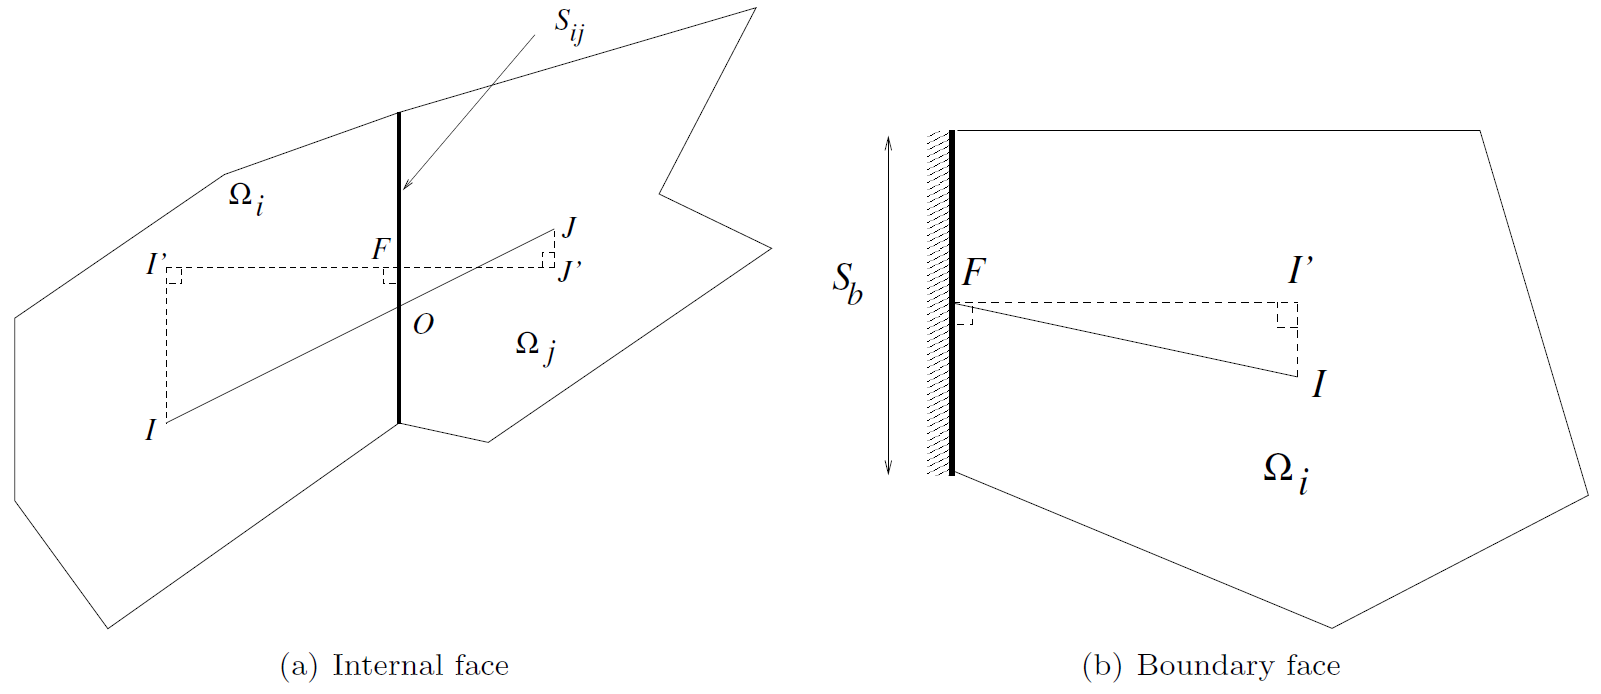
\includegraphics[width=\textwidth]{./images/cell_face.png}
\caption{
Quantities used in the finite volume discretization.
Left: cell $\Omega_i$, cell $\Omega_j$ and the internal face $S_{ij}$ connecting them.
Right: boundary cell $\Omega_i$ and associated boundary face $S_b$.
{\fontfamily{ppl}\fontshape{it}\selectfont Code\_Saturne} 5.0.0 theory guide \cite{saturne2017}.
}\label{fig-cell_face}
\end{figure}

For an internal face --- i.e. $S_{ij}$ ---, the thermal flux from cell $\Omega_i$ to cell $\Omega_j$ per unit surface, written $D_{ij}$, is
\begin{equation}
\label{eq-dij}
D_{ij} = \lambda_{ij} \frac{T_{J'}-T_{I'}}{I'J'}
\end{equation}
where $\lambda_{ij}$ is the thermal conductivity on the internal face $S_{ij}$.
For a boundary face --- i.e. $S_b$ ---, the thermal flux out of cell $\Omega_i$ per unit surface, written $D_{ib}$, is
\begin{equation}
\label{eq-dib}
D_{ib} = \lambda_i \frac{T_{F}-T_{I'}}{I'F}
\end{equation}
Thus, the thermal flux from a boundary face to a neighbouring cell $\Omega_j$ per unit surface, written $D_{bj}$, is
\begin{equation}
\label{eq-dbj}
D_{bj} = \lambda_j \frac{T_{J'}-T_{F}}{FJ'}
\end{equation}
If the field is coupled, the fluxes per unit surface $D_{ib}$ and $D_{bj}$ are equal.
This flux will be written $D_{ibj}$.
The faces temperature $T_F$ in equations (\ref{eq-dib}) and (\ref{eq-dbj}) are also equal.
This leads to
\begin{equation}
\left( \frac{F J'}{\lambda_j} + \frac{I' F}{\lambda_i} \right) D_{ibj} = \left( T_{J'}-T_{I'} \right)
\end{equation}
To conclude, the flux $D_{ibj}$ of the coupled field should be equal to the flux $D_{ij}$ we would have obtained on an internal face.
Thus, using equation (\ref{eq-dij}) and writing $\eta_{ij} = \frac{I' F}{I' J'}$, one gets
\begin{equation}
\frac{1}{\lambda_{ij}} = \left( \frac{1-\eta_{ij}}{\lambda_j} + \frac{\eta_{ij}}{\lambda_i} \right)
\end{equation}
This demonstrates that an harmonic interpolation for the face thermal conductivity gives a fully conservative coupling strategy.
Second order accuracy in space on non-orthogonal meshes is reached thanks to an iterative process.

The main advantage of the present coupling strategy is that the solver remains fully conservative in case of conjugate heat transfer.
In addition, second-order accuracy in time is preserved.
The main disadvantage is that the velocity and the pressure are also defined in the solid domains.
As both remain exactly zero inside the solid, this is not an issue, but it does lead to higher memory usage compared with a dedicated solver for the solid thermal diffusion.
This coupling strategy will provide a valuable framework for future RANS models able to tackle conjugate heat transfer.
%It should also be noted that the current implementation is not compatible with the multigrid solver.

\section{Impact of the SGS model and $Pr_t$}
\label{sec-sgs_appendix}

Prior to the present study, several LES of a turbulent channel flow at $Re_\tau=1020$ were performed to select a SGS model for the momentum equation.
The mesh used corresponds exactly to the one described in the Subsection \ref{subsec-geom}.
SGS models tested already implemented in Code\_Saturne were the Standard Smagorinsky ($Std.Smag$), the WALE model ($Wale$), and 2 variants of the Dynamic Smagorinsky ($Dyn.Smag.1$ and $Dyn.Smag.2$).
The two variants of the Dynamic Smagorinsky SGS model are using different clippings.
The authors also tested some variants of the Dynamic Smagorinsky model with spatial averaging over homogeneous directions.
As they did not bring significant improvements, they are simply omitted here.

\begin{figure}[hbp]
\centering
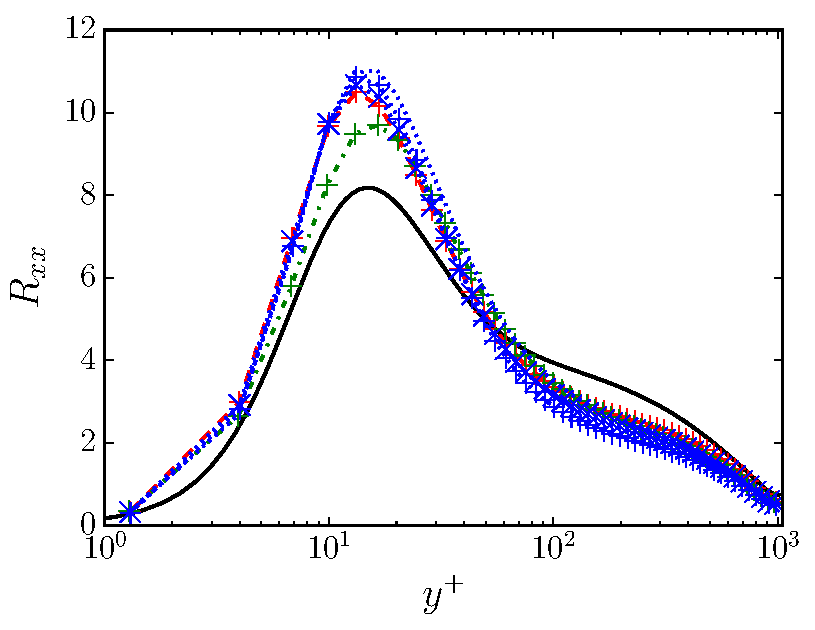
\includegraphics[width=\textwidth]{./appendix_re_1020/plots/rxx.pdf}
\caption{
LES of a turbulent channel flow at $Re_\tau=1020$.
Impact of the SGS model on the variance of the streamwise velocity.
}\label{fig-sgs_rxx}
\end{figure}

\begin{figure}
\centering
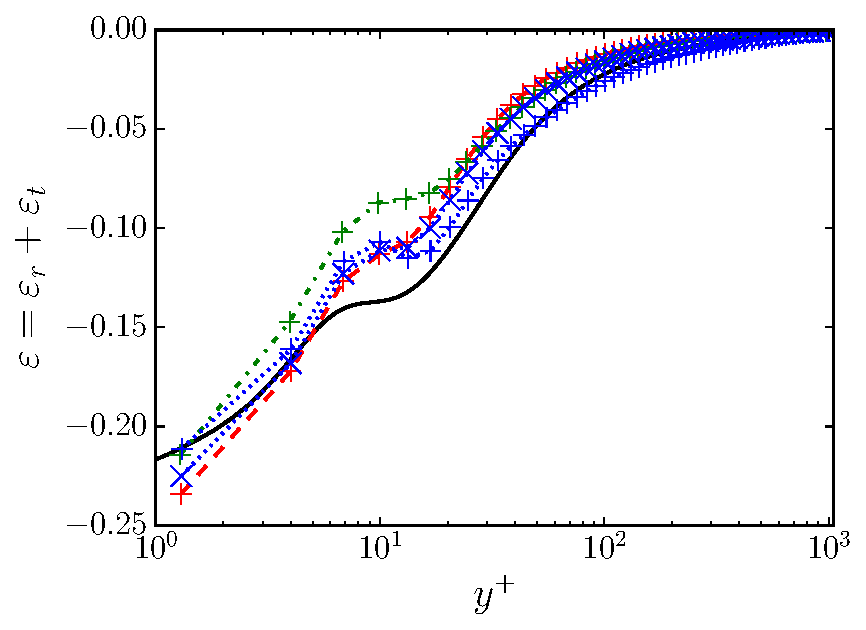
\includegraphics[width=\textwidth]{./appendix_re_1020/plots/diss.pdf}
\caption{
LES of a turbulent channel flow at $Re_\tau=1020$.
Impact of the SGS model on the dissipation rate associated with the turbulent kinetic energy.
}\label{fig-sgs_diss}
\end{figure}

Overall, the SGS models tested only provide a qualitative agreement for the Reynolds stresses. 
This is illustrated in Figure \ref{fig-sgs_rxx} with the variance of the streamwise velocity ($\overline{{u'_x}^2}$).
Regarding the dissipation rate ($\varepsilon$) associated with the turbulent kinetic energy, Figure \ref{fig-sgs_diss} shows that the $Wale$ SGS model provides the best estimation near the wall.
The $Wale$ SGS model was selected on this criterion.

\begin{figure}
\centering
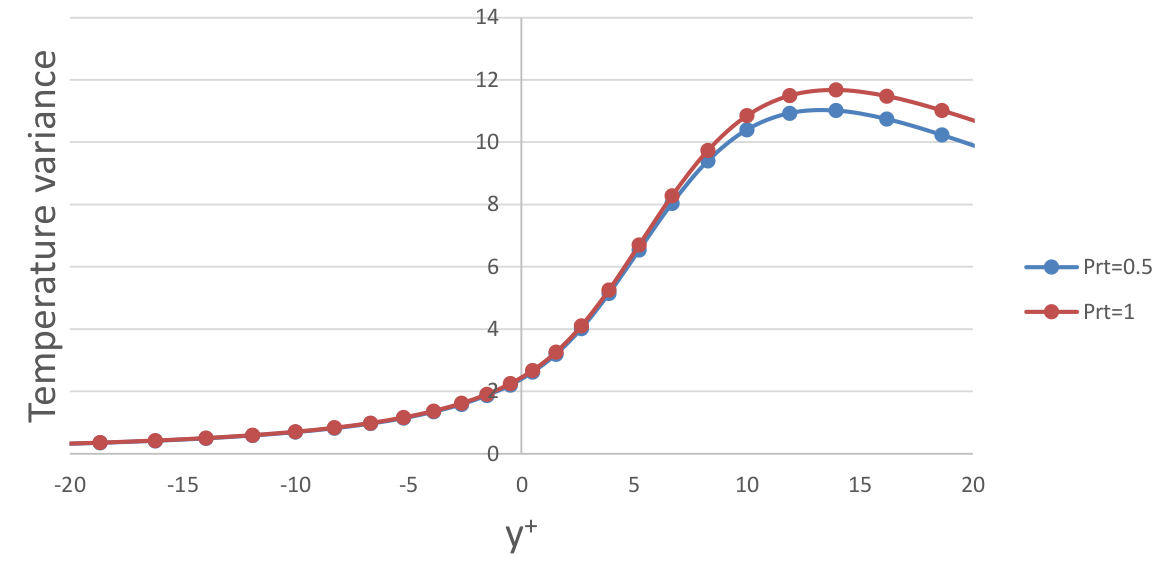
\includegraphics[width=\textwidth]{./images/impact_Prt_TT.png}
\caption{
LES of a turbulent channel flow at $Re_\tau=395$ and $Pr=1$.
Conjugate heat transfer with $K = G = G_2 = 1$.
Impact of the turbulent Prandtl number ($Pr_t$) on the variance of the temperature.
}\label{fig-sgs_tt}
\end{figure}

\begin{figure}
\centering
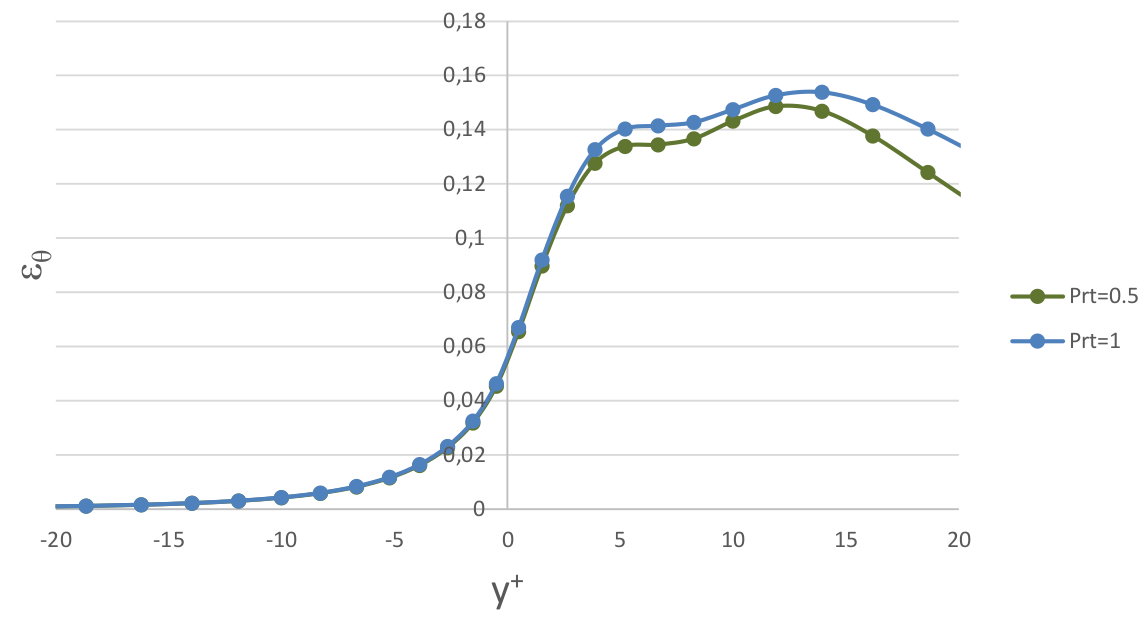
\includegraphics[width=\textwidth]{./images/impact_Prt_dissTT.png}
\caption{
LES of a turbulent channel flow at $Re_\tau=395$ and $Pr=1$.
Conjugate heat transfer with $K = G = G_2 = 1$.
Impact of the turbulent Prandtl number ($Pr_t$) on $\varepsilon_\theta$.
}\label{fig-sgs_disstt}
\end{figure}

The authors have also looked at the impact of the turbulent Prandtl number ($Pr_t$).
Two simulations were performed at $Re_\tau = 395$ and $Pr = 1$ using conjugate heat transfer with unit ratios of fluid-solid thermal properties ($K = G = G_2 = 1$).
The mesh used corresponds exactly to the one described in the Subsection \ref{subsec-geom}.
One simulation were performed with $Pr_t = 0.5$ and the other with $Pr_t = 1$.
As visible on Figures \ref{fig-sgs_tt} and \ref{fig-sgs_disstt}, the turbulent Prandtl number has no significant impact on the statistics in the near-wall layer ($y^+ < 5$).

When performing a LES, the choice of the SGS models used in the momentum equation and in the energy equation is of paramount importance.
However, development and testing of refined SGS models is out of the scope of the present study.
Thus, the authors have decided to combine a fine mesh with relatively simple SGS models already implemented in Code\_Saturne, and to carefully assess the obtained results using DNS.

\end{document}
